\chapter{双层优化}
\label{chap:bilevel-optimization}

用一个数$x\geq0$控制一次拟合的保守程度：$x$越大，拟合结果越被压向零。对每个$x$，先解一个拟合问题，得到结果$y$；再拿$y$和另一个固定的数比较，判断$x$选得好不好。要评价一个$x$，必须先完成一次优化。这样的问题里，决策分成两层，上面一层的目标要读取下面一层的最优解。

这种嵌套带来三个问题。第一，下面一层可能无解，也可能有许多个同样好的解，“把内解代入外层”这句话要先说清选的是哪一个。第二，外层要下降就要知道目标对$x$的导数，而内解没有显式公式。第三，所有计算都只是近似，内层没解准、线性方程没解准、外层没走完，这几种误差要分开核算。

本章依次回答这三个问题。第~\ref{sec:bilevel-problem}节确定数学对象，区分唯一内解、多解选择和有限步输出。第~\ref{sec:bilevel-solution-map}节检查内解能否沿一条分支光滑变化，以及分支在什么地方断开。第~\ref{sec:bilevel-implicit}节和第~\ref{sec:bilevel-unrolling}节给出两种求导路线，前者只看解点处的方程，后者沿算法的每一步传播导数。第~\ref{sec:bilevel-single-level}节换一种思路，把内层最优性写成约束。第~\ref{sec:bilevel-outer}节把三类误差放在一起，给出外层的求解和停止依据。

\section{双层问题}
\label{sec:bilevel-problem}

外层目标依赖内层的最优解时，它到底是一个什么样的函数？先把两层的角色写下来。

外层变量记为$\bm{x}\in\bm{C}\subseteq\mathbb{R}^n$，内层变量记为$\bm{y}\in\mathbb{R}^d$。外层选定$\bm{x}$之后，内层在可行集$\bm{Y}(\bm{x})\subseteq\mathbb{R}^d$上最小化自己的目标$g$；外层再用另一个目标$F$评价内层的结果。

\begin{definition}[内层解集]
\label{def:bilevel-inner-solutions}
给定$\bm{x}\in\bm{C}$，称
\begin{equation}
 \bm{S}(\bm{x})=\argmin_{\bm{y}\in\bm{Y}(\bm{x})}g(\bm{x},\bm{y})
 \label{eq:bilevel-solution-set}
\end{equation}
为\term{内层解集}（lower-level solution set），其中的点称为内解。外层目标$F(\bm{x},\bm{y})$只对内解作评价，由此形成的嵌套问题称为\term{双层优化}（bilevel optimization）问题。
\end{definition}

图~\ref{fig:bilevel-structure}是这个结构的全貌。$\bm{x}$有两条路影响外层：一条直接进入$F$，另一条先改变内层问题，再通过选出的内解起作用。外层只能修改$\bm{x}$，不能直接修改$\bm{y}$。中间的“选解规则”一格是定义里没有出现、却必不可少的一步，第~\ref{sec:bilevel-selection}小节会讲它。

\begin{BookInlineFigure}
 \centering
 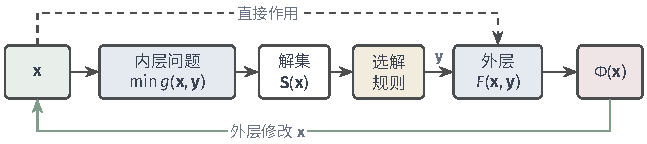
\includegraphics[width=109.6mm]{figures/05-optimization/07-multiple-criteria-and-nested-optimization/tikz/bilevel-structure/figure.pdf}
 \caption{双层问题的结构。外层变量$\bm{x}$决定内层问题，内层解集经选解规则给出$\bm{y}$，外层目标$F$再读取$\bm{y}$得到$\Phi(\bm{x})$。虚线是$\bm{x}$对$F$的直接作用，绿线表示外层根据$\Phi$修改$\bm{x}$。}
 \label{fig:bilevel-structure}
\end{BookInlineFigure}

\paragraph{内层无解时外层没有输入}
解集可能是空集。取外层变量$x\in\mathbb{R}$，内层变量$y\in\mathbb{R}$，内层目标是
\[
 g(x,y)=\frac{x}{2}y^2-y.
\]

$x>0$时这是开口向上的抛物线，唯一的内解是$y=1/x$。$x=0$时$g=-y$，$x<0$时$g$是开口向下的抛物线，两种情况下$y\to+\infty$都使$g\to-\infty$，内层没有最小点。

这时一个内层算法仍然可以运行并输出数字。比如梯度下降的更新是$y\leftarrow y+\alpha(1-xy)$，在$x<0$时迭代会不断增大。把这种数字交给外层，得到的外层值不评价任何内解。因此外层只在下面的集合上比较：
\begin{equation}
 \operatorname{dom}\bm{S}=\{\bm{x}\in\bm{C}:\bm{S}(\bm{x})\neq\varnothing\}.
 \label{eq:bilevel-dom}
\end{equation}
集合之外的$\bm{x}$一律视为外层不可行，外层值规定为$+\infty$。

\paragraph{与极小极大的区别}
第~\ref{chap:minimax-optimization}章的问题$\min_{\bm{x}}\max_{\bm{y}}f(\bm{x},\bm{y})$也是嵌套的，形式上取$g=-f$、$F=f$就是双层问题。可是那里两层围绕同一个代价相反地优化，内层的最优性恰好让外层目标对$\bm{y}$的偏导为零。双层问题的两个目标一般无关，内层最优并不让$F$在$\bm{y}$方向驻定，内解移动一点，外层值就跟着变化。表~\ref{tab:bilevel-vs-minimax}对比两者，第~\ref{sec:bilevel-hypergradient}小节会用公式说明最后一行。

\begin{BookInlineTable}
 \centering
 \begin{tabular}{lll}
  \toprule
  & 极小极大 & 双层优化\\
  \midrule
  内外目标 & 同一个$f$，方向相反 & $g$与$F$一般无关\\
  内解处$\nabla_{\bm{y}}F$ & 为零 & 一般不为零\\
  外层导数 & 无需内解的响应项 & 必须计入内解的响应\\
  \bottomrule
 \end{tabular}
 \caption{极小极大与双层优化的对比。第二、三行假定内解唯一、位于内层可行集内部且相关函数可微。}
 \label{tab:bilevel-vs-minimax}
\end{BookInlineTable}

\subsection{唯一内解}
\label{sec:bilevel-unique}

最简单的情形是对每个$\bm{x}$，解集恰有一个点，$\bm{S}(\bm{x})=\{\bm{y}^\star(\bm{x})\}$。这时选解不成问题，外层目标是一个普通的函数。

\begin{definition}[外层目标]
\label{def:bilevel-outer}
设对每个$\bm{x}\in\bm{C}$内解唯一，记为$\bm{y}^\star(\bm{x})$。外层问题是在$\bm{C}$上最小化
\begin{equation}
 \Phi(\bm{x})=F(\bm{x},\bm{y}^\star(\bm{x})).
 \label{eq:bilevel-phi}
\end{equation}
\end{definition}

$\Phi$的变化有两个来源。$\bm{x}$变动时，$F$的第一个位置直接变，这是直接作用；$\bm{y}^\star(\bm{x})$随之移动，$F$的第二个位置也变，这是响应。后者才是双层问题的特点，第~\ref{sec:bilevel-implicit}节专门计算它。

\paragraph{贯穿全章的正则拟合例}
下面的例子贯穿全章。内层用观测值$3$拟合一个数$y$，并用$x\geq0$惩罚$y$的大小；外层把结果和另一个固定的数$1$比较：
\begin{equation}
 g(x,y)=\frac12(y-3)^2+\frac{x}{2}y^2,\qquad F(x,y)=\frac12(y-1)^2.
 \label{eq:bilevel-ridge}
\end{equation}

对$y$求导并令导数为零，得到$(1+x)y-3=0$。$x\geq0$时$g$对$y$的二阶导数是$1+x>0$，所以内解唯一：
\begin{equation}
 y^\star(x)=\frac{3}{1+x}.
 \label{eq:bilevel-ridge-solution}
\end{equation}

代入式~\eqref{eq:bilevel-phi}，外层目标是
\[
 \Phi(x)=\frac12\Bigl(\frac{3}{1+x}-1\Bigr)^2.
\]
当$x=2$时内解恰好等于$1$，$\Phi$取到最小值$0$。

\paragraph{两个目标为什么不能合并}
看图~\ref{fig:bilevel-reaction}(a)。粗线是$y^\star(x)$的图像，只有粗线上的点才算内层最优。若把$x$和$y$一起放进$g$里最小化，得到的是空心点$(0,3)$，因为惩罚对$g$只是一种代价，$g$总愿意取$x=0$。若把两者一起放进$F$里最小化，虚线$y=1$上每一点都是最优的，$x$完全不起作用，等于直接把拟合结果改成想要的数。

双层结构要求的是第三种做法：沿粗线走，在粗线上找$F$最小的点。这正像预算线上的最优：可选的点被限制在一条曲线上，只不过这条曲线本身要靠解优化问题才能画出来。图~\ref{fig:bilevel-reaction}(b)把粗线上的外层值画成$x$的函数，最小点在$x=2$。

\begin{BookInlineFigure}
 \centering
 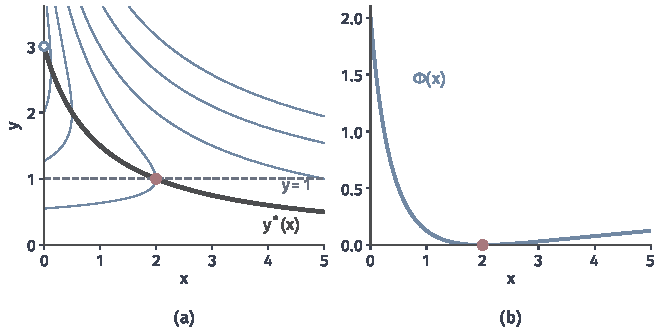
\includegraphics[width=112mm]{figures/05-optimization/07-multiple-criteria-and-nested-optimization/matplotlib/bilevel-reaction/figure.pdf}
 \caption{正则拟合例~\eqref{eq:bilevel-ridge}。(a)蓝色细线是内层目标$g$的等高线，空心点$(0,3)$是$g$对$(x,y)$的最小点；深灰粗线是内解曲线$y^\star(x)=3/(1+x)$；虚线$y=1$上$F$取最小值；红点$(2,1)$是双层问题的解。(b)外层目标$\Phi(x)$，最小点是$x=2$。}
 \label{fig:bilevel-reaction}
\end{BookInlineFigure}

\paragraph{直接作用的例子}
式~\eqref{eq:bilevel-ridge}中$F$不含$x$，全部变化都来自响应。若外层再为$x$付出代价，比如把$F$换成$\frac12(y-1)^2+\frac{1}{10}x$，直接作用就出现了：$\Phi$多了一项$\frac{1}{10}x$，最小点从$x=2$向左移动。两个来源在导数中分别对应一项。

这里的$3$和$1$只是两个固定的数，本章把它们当作给定的优化数据。数据该怎样划分，这样选出的$x$有没有统计上的保证，不是优化问题，可参考\BookChapterRef{chap:finite-sample-error-bounds}{卷八第4章“有限样本的误差上界”}。

\subsection{多解选择}
\label{sec:bilevel-selection}

解集可能含有许多点，它们对内层来说一样好，对外层却可能差别很大。这时$F(\bm{x},\bm{y}^\star(\bm{x}))$这个写法失去了意义，必须补充一条规则。

\paragraph{两种选解规则}
可以用一个比喻来理解。外层是提要求的一方，内层是执行的一方，执行方在几个同样好的方案之间不在乎选哪个。外层可以假定执行方会配合自己，也可以防备它选最不利的。这个比喻只用来记住两种规则，数学上并不要求内层真有什么意愿，规则只是对解集中的点作出约定。

\begin{definition}[乐观模型与悲观模型]
\label{def:bilevel-opt-pes}
对$\bm{x}\in\operatorname{dom}\bm{S}$，定义
\begin{align}
 \Phi_{\mathrm{o}}(\bm{x})&=\inf_{\bm{y}\in\bm{S}(\bm{x})}F(\bm{x},\bm{y}),
 \label{eq:bilevel-optimistic}\\
 \Phi_{\mathrm{p}}(\bm{x})&=\sup_{\bm{y}\in\bm{S}(\bm{x})}F(\bm{x},\bm{y}),
 \label{eq:bilevel-pessimistic}
\end{align}
对$\bm{x}\notin\operatorname{dom}\bm{S}$，两者都规定为$+\infty$。在$\bm{C}$上最小化$\Phi_{\mathrm{o}}$称为\term{乐观模型}（optimistic model），最小化$\Phi_{\mathrm{p}}$称为\term{悲观模型}（pessimistic model）。
\end{definition}

空集上的规定要单独写出。按惯例$\sup\varnothing=-\infty$，若照搬，内层无解的$\bm{x}$在悲观模型中外层值是$-\infty$，反而成了最好的选择，这与第~\ref{sec:bilevel-problem}节开头的约定相反。

两个函数处处满足$\Phi_{\mathrm{o}}\leq\Phi_{\mathrm{p}}$，内解唯一时都等于$\Phi$。乐观模型的$\inf$可以和外层的$\inf$合并，于是
\begin{equation}
 \inf_{\bm{x}\in\bm{C}}\Phi_{\mathrm{o}}(\bm{x})=\inf\{F(\bm{x},\bm{y}):\bm{x}\in\bm{C},\ \bm{y}\in\bm{S}(\bm{x})\}.
 \label{eq:bilevel-optimistic-joint}
\end{equation}
乐观模型因而是一个对$(\bm{x},\bm{y})$的联合最小化，可行集是解集的图像。悲观模型夹着一层$\sup$，不能这样合并。

\paragraph{一个手算例子}
取$\bm{C}$和内层可行集都是$[-1,1]$，目标是
\[
 g(x,y)=xy,\qquad F(x,y)=x^2+y.
\]

内层在$[-1,1]$上最小化关于$y$的线性函数，解由$x$的符号决定：
\[
 S(x)=\begin{cases}
 \{1\}, & x<0,\\
 [-1,1], & x=0,\\
 \{-1\}, & x>0.
 \end{cases}
\]

$x\neq0$时只有一个内解，两种模型相同：$x<0$时外层值是$x^2+1$，$x>0$时外层值是$x^2-1$。分歧只在$x=0$，此时整个区间都是内解，$F(0,y)=y$，于是
\[
 \Phi_{\mathrm{o}}(0)=-1,\qquad\Phi_{\mathrm{p}}(0)=1.
\]

图~\ref{fig:bilevel-selection}画出了这个例子。乐观模型在$x=0$取到最小值$-1$，红点就是它的解。悲观模型的下确界同样是$-1$，因为$x\downarrow0$时$x^2-1\to-1$，但这个值取不到：$x=0$处值跳到$1$，$x>0$时值严格大于$-1$。悲观模型没有最优解。

\begin{BookInlineFigure}
 \centering
 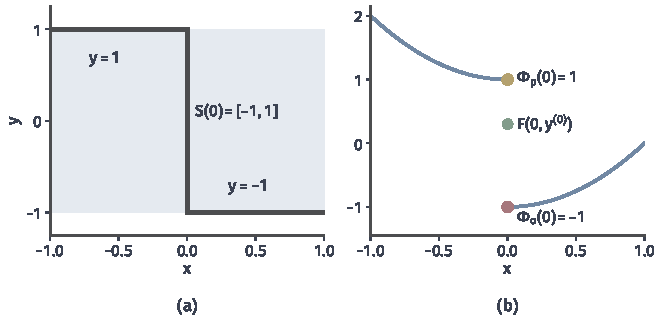
\includegraphics[width=112mm]{figures/05-optimization/07-multiple-criteria-and-nested-optimization/matplotlib/bilevel-selection/figure.pdf}
 \caption{多解时的选解。内层$g=xy$，$x,y\in[-1,1]$，外层$F=x^2+y$。(a)浅蓝是内层可行集，深灰线是解集$S(x)$的图像，$x=0$处是整段区间。(b)蓝线是$x\neq0$时共同的外层值。$x=0$处，红点是乐观值，黄点是悲观值，绿点是从$y^{(0)}=0.3$出发的投影梯度法实际得到的外层值。}
 \label{fig:bilevel-selection}
\end{BookInlineFigure}

\paragraph{乐观模型的解存在，悲观模型没有这样的保证}
上例不是偶然的。把式~\eqref{eq:bilevel-optimistic-joint}看成解集图像上的最小化，就可以套用第~\ref{chap:optimization}章的存在定理，只需说明图像是紧的。

\begin{theorem}[乐观模型解的存在]
\label{thm:bilevel-optimistic-existence}
设$\bm{C}$和$\bm{Y}$是非空紧集，内层可行集恒为$\bm{Y}$，$g$和$F$在$\bm{C}\times\bm{Y}$上连续。则集合
\begin{equation}
 \bm{G}=\{(\bm{x},\bm{y}):\bm{x}\in\bm{C},\ \bm{y}\in\bm{S}(\bm{x})\}
 \label{eq:bilevel-graph}
\end{equation}
非空且紧，乐观模型有最优解。
\end{theorem}

\begin{proof}
对每个$\bm{x}\in\bm{C}$，连续函数$g(\bm{x},\cdot)$在紧集$\bm{Y}$上取得最小值，所以$\bm{S}(\bm{x})$非空，$\bm{G}$非空。$\bm{G}$含于紧集$\bm{C}\times\bm{Y}$，只需证明它是闭集。

取$\bm{G}$中收敛到$(\bm{x},\bm{y})$的序列$(\bm{x}^{(k)},\bm{y}^{(k)})$。$\bm{C}$、$\bm{Y}$闭，所以$\bm{x}\in\bm{C}$，$\bm{y}\in\bm{Y}$。任取比较点$\bm{z}\in\bm{Y}$，由$\bm{y}^{(k)}$是内解，有
\[
 g(\bm{x}^{(k)},\bm{y}^{(k)})\leq g(\bm{x}^{(k)},\bm{z}).
\]

令$k\to\infty$，由$g$连续，得到
\[
 g(\bm{x},\bm{y})\leq g(\bm{x},\bm{z}).
\]
$\bm{z}$是任取的，所以$\bm{y}\in\bm{S}(\bm{x})$，$\bm{G}$是闭集。连续函数$F$在紧集$\bm{G}$上取得最小值，由式~\eqref{eq:bilevel-optimistic-joint}，它就是乐观模型的最优值。
\end{proof}

前面的例子满足定理的全部条件，悲观模型却没有解。原因是第~\ref{chap:optimization}章存在论证的第三关：悲观目标在$x=0$处向上跳，不是下半连续的。

\paragraph{算法的隐含择解}
实际运行时，算法既不会自动做$\inf$，也不会自动做$\sup$。上例中$x=0$时内层梯度是$\partial_yg=x=0$，投影梯度法根本不动，停在初值。从$y^{(0)}=0.3$出发，得到外层值$F(0,0.3)=0.3$，这就是图~\ref{fig:bilevel-selection}(b)的绿点，它既不是乐观值，也不是悲观值。

所以声称求解某个模型时，要说清算法的输出怎样对应这个模型；对应不上的话，算出来的只是“这个算法从这个初值给出的外层值”。

\subsection{有限步内解}
\label{sec:bilevel-finite}

精确内解通常拿不到，实际手里的是算法运行若干步的结果。这个结果也是$\bm{x}$的函数，但它和内解是不同的对象。

\begin{definition}[有限步目标]
\label{def:bilevel-finite}
给定内层算法的初始化和更新规则，把运行$T$步的输出记为$\bm{y}^{(T)}(\bm{x})$。称
\begin{equation}
 \Phi_T(\bm{x})=F(\bm{x},\bm{y}^{(T)}(\bm{x}))
 \label{eq:bilevel-finite-objective}
\end{equation}
为\term{有限步目标}（finite-step objective）。
\end{definition}

这个函数依赖初值、更新规则、步长和步数，换掉任何一项就是另一个函数。

\paragraph{用正则拟合例计算}
对式~\eqref{eq:bilevel-ridge}的内层用梯度下降，初值$y^{(0)}=0$，步长$\alpha=1/2$。内层梯度是$(1+x)y-3$，代入更新式，得到
\[
 y^{(t+1)}=y^{(t)}-\frac12\bigl[(1+x)y^{(t)}-3\bigr]=q\,y^{(t)}+\frac32,\qquad q=\frac{1-x}{2}.
\]

减去不动点$y^\star(x)$，误差每步乘$q$，初始误差是$-y^\star(x)$，所以
\begin{equation}
 y^{(T)}(x)=y^\star(x)\bigl(1-q^T\bigr).
 \label{eq:bilevel-ridge-finite}
\end{equation}

$T$较小时可以写成多项式。前两步的结果是
\[
 y^{(1)}=\frac32,\qquad y^{(2)}=\frac94-\frac34x.
\]

$y^{(1)}$与$x$无关，于是$\Phi_1$是常数，走一步完全看不到$x$的作用。$\Phi_2$的最小点由$y^{(2)}=1$确定，得到$x=5/3$，与$\Phi$的最小点$x=2$不同。

再看$T=3$。直接计算得$y^{(3)}=\frac32(q^2+q+1)$，它在$q=-1/2$时最小，最小值是$9/8$。这时$y^{(3)}$到不了$1$，$\Phi_3$的最小点是$x=2$，最小值却是$1/128$，不是$0$。图~\ref{fig:bilevel-finite-step}比较了几个$T$。

\begin{BookInlineFigure}
 \centering
 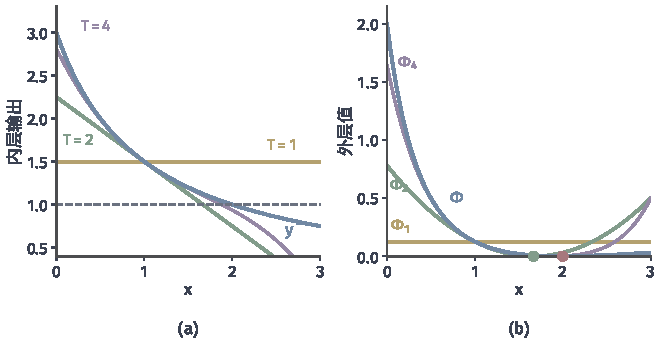
\includegraphics[width=112mm]{figures/05-optimization/07-multiple-criteria-and-nested-optimization/matplotlib/bilevel-finite-step/figure.pdf}
 \caption{有限步内解与有限步目标，内层梯度下降取$y^{(0)}=0$、$\alpha=1/2$。(a)内层输出$y^{(T)}(x)$（$T=1,2,4$）与精确内解$y^\star(x)$（蓝）；所有曲线在$x=1$相交，因为此时$q=0$，一步即得精确解。(b)对应的$\Phi_T$与$\Phi$。绿点是$\Phi_2$的最小点$x=5/3$，红点是$\Phi$的最小点$x=2$。}
 \label{fig:bilevel-finite-step}
\end{BookInlineFigure}

\paragraph{设计目标还是近似手段}
这里要区分两种立场。第一种，最终交付的就是“运行$T$步的这个过程”，$T$和初值是设计的一部分，那么$\Phi_T$本身就是要优化的目标，它的梯度是精确的，不必谈$\bm{y}^\star$。第二种，真正关心的是最优选解，$T$步只是不得已的近似，那么$\Phi_T$与$\Phi$的差别就是要核算的误差。

两种立场下同一个数字含义不同，不能因为运行的是优化算法，就把$\bm{y}^{(T)}(\bm{x})$称作$\bm{y}^\star(\bm{x})$。表~\ref{tab:bilevel-objects}列出本节得到的三个对象。

\begin{BookInlineTable}
 \centering
 \begin{tabular}{lll}
  \toprule
  对象 & 需要说明什么 & 依赖\\
  \midrule
  内解唯一的$\Phi$ & 唯一性 & 问题本身\\
  $\Phi_{\mathrm{o}}$、$\Phi_{\mathrm{p}}$ & 乐观或悲观 & 问题与规则\\
  $\Phi_T$ & 初值、更新、步数 & 算法实现\\
  \bottomrule
 \end{tabular}
 \caption{外层目标的三种对象。内层无解的$\bm{x}$不属于前两行的讨论范围。}
 \label{tab:bilevel-objects}
\end{BookInlineTable}

\section{内层解映射}
\label{sec:bilevel-solution-map}

外层要下降，需要知道$\Phi$的导数，而$\Phi$里含着内解。内解能不能看成$\bm{x}$的光滑函数？这个问题要分范围回答，因为“内解”可以指三种不同范围的东西：全局解集、某个局部极小点所在的分支，以及只满足驻点方程的点。

第~\ref{chap:parametric-sensitivity}章已经研究过解随参数的变化。本节把那里的结论放到双层语境中使用：先确定追踪的是哪个范围的分支，再讨论能否对它求导。

\subsection{可微分支}
\label{sec:bilevel-branch}

先看无约束内层，$\bm{Y}(\bm{x})=\mathbb{R}^d$。内层的碗底满足驻点方程$\nabla_{\bm{y}}g=\bm{0}$。外层变量一动，碗的形状变化，碗底跟着移动，移动多少由碗的曲率决定：曲率大的方向，碗底只需挪一点就能抵消梯度的变化。

\paragraph{局部分支}
记$(\bm{x}_0,\bm{y}_0)$为基准点。下面的定理就是第~\ref{chap:parametric-sensitivity}章的无约束解导数定理，这里按双层记号复述。

\begin{theorem}[局部极小分支]
\label{thm:bilevel-local-branch}
设$g$在$(\bm{x}_0,\bm{y}_0)$的邻域内二阶连续可微，$\nabla_{\bm{y}}g(\bm{x}_0,\bm{y}_0)=\bm{0}$，且$\nabla^2_{\bm{y}\bm{y}}g(\bm{x}_0,\bm{y}_0)\succ\bm{0}$。则存在$\bm{x}_0$的邻域$\bm{U}$、$\bm{y}_0$的邻域$\bm{V}$和唯一的连续可微映射$\hat{\bm{y}}:\bm{U}\to\bm{V}$，使$\hat{\bm{y}}(\bm{x}_0)=\bm{y}_0$，并且对$\bm{x}\in\bm{U}$有
\begin{equation}
 \nabla_{\bm{y}}g(\bm{x},\hat{\bm{y}}(\bm{x}))=\bm{0},
 \label{eq:bilevel-branch-stationary}
\end{equation}
每个$\hat{\bm{y}}(\bm{x})$都是$g(\bm{x},\cdot)$的严格局部极小点。其Jacobian矩阵为
\begin{equation}
 \bm{D}(\bm{x})=\frac{\partial\hat{\bm{y}}}{\partial\bm{x}}=-\bm{H}^{-1}\bm{B},
 \label{eq:bilevel-branch-derivative}
\end{equation}
其中$\bm{H}=\nabla^2_{\bm{y}\bm{y}}g$是$d\times d$矩阵，$\bm{B}=\nabla^2_{\bm{y}\bm{x}}g$是$d\times n$矩阵，其$(i,j)$元素是$\partial^2g/\partial y_i\partial x_j$，两者都在$(\bm{x},\hat{\bm{y}}(\bm{x}))$处取值。
\end{theorem}

\begin{proof}
把驻点方程$\nabla_{\bm{y}}g(\bm{x},\bm{y})=\bm{0}$看成$d$个方程、$d$个未知量$\bm{y}$、参数$\bm{x}$的系统。它对$\bm{y}$的Jacobian矩阵是$\bm{H}$，在基准点正定，因而可逆。隐函数定理给出邻域和唯一的连续可微分支，定理的陈述可参考\BookChapterRef{chap:implicit-inverse-functions}{卷二第22章“隐函数与反函数”}。

沿分支式~\eqref{eq:bilevel-branch-stationary}恒成立，对$\bm{x}$求导，得到
\[
 \bm{H}\bm{D}+\bm{B}=\bm{0},
\]
这就是式~\eqref{eq:bilevel-branch-derivative}。

Hessian连续，矩阵最小特征值连续依赖矩阵，所以缩小$\bm{U}$后沿分支$\bm{H}\succ\bm{0}$。驻点处Hessian正定，由二阶充分条件，$\hat{\bm{y}}(\bm{x})$是严格局部极小点。
\end{proof}

定理的三个条件各有作用。二阶连续可微使驻点方程本身连续可微。驻点方程保证基准点在分支上。Hessian正定有两份工作：它的可逆性给出分支，它的正定性保证分支上的点是极小点而不是别的驻点。

结论是局部的。定理说的是基准点附近有一条光滑的局部极小点曲线，没有说这些点是内层的全局最优解，所以这时的$\hat{\bm{y}}(\bm{x})$还不能当作$\bm{S}(\bm{x})$中的点。

\paragraph{全局强凸时分支就是唯一内解}
要让分支代表全局内解，需要全局的条件。强凸是最常用的一个。

\begin{theorem}[强凸内层的解映射]
\label{thm:bilevel-strong-convex-map}
设$\bm{U}\subseteq\mathbb{R}^n$开，$\bm{Y}(\bm{x})=\mathbb{R}^d$，$g$在$\bm{U}\times\mathbb{R}^d$上二阶连续可微，且存在$\mu>0$，使$\nabla^2_{\bm{y}\bm{y}}g\succeq\mu\bm{I}$处处成立。则对每个$\bm{x}\in\bm{U}$，内解存在且唯一，$\bm{y}^\star$在$\bm{U}$上连续可微，其Jacobian矩阵$\bm{D}$由式~\eqref{eq:bilevel-branch-derivative}给出，并满足
\begin{equation}
 \lVert\bm{D}(\bm{x})\rVert_2\leq\frac{\lVert\bm{B}\rVert_2}{\mu}.
 \label{eq:bilevel-map-lipschitz}
\end{equation}
\end{theorem}

\begin{proof}
固定$\bm{x}\in\bm{U}$，把$g(\bm{x},\cdot)$简写成$\phi$。由带积分余项的Taylor公式和Hessian下界，对任意$\bm{y},\bm{z}$有
\[
 \phi(\bm{z})\geq\phi(\bm{y})+\langle\nabla\phi(\bm{y}),\bm{z}-\bm{y}\rangle+\frac{\mu}{2}\lVert\bm{z}-\bm{y}\rVert_2^2.
\]

取$\bm{y}=\bm{0}$，右端随$\lVert\bm{z}\rVert_2\to\infty$趋于$+\infty$，所以下水平集有界。$\phi$连续，下水平集也是闭集，因而紧。由第~\ref{chap:optimization}章的紧下水平集存在定理，最小点存在。

若$\bm{y}$是驻点，上面的不等式给出$\phi(\bm{z})>\phi(\bm{y})$对一切$\bm{z}\neq\bm{y}$成立。所以驻点就是唯一的全局最小点，内解唯一。

任取$\bm{x}_0\in\bm{U}$，定理~\ref{thm:bilevel-local-branch}在$(\bm{x}_0,\bm{y}^\star(\bm{x}_0))$处给出局部分支$\hat{\bm{y}}$。分支上的点都是驻点，而驻点就是内解，所以在$\bm{x}_0$附近$\hat{\bm{y}}=\bm{y}^\star$。因此$\bm{y}^\star$连续可微，导数公式成立。由$\bm{H}\succeq\mu\bm{I}$得$\lVert\bm{H}^{-1}\rVert_2\leq1/\mu$，这就给出式~\eqref{eq:bilevel-map-lipschitz}。
\end{proof}

对正则拟合例，$g$对$y$的二阶导数是$1+x$，在开集$x>-1/2$上不小于$\mu=1/2$，定理适用，在$x\geq0$上还可以取$\mu=1$。这里$B=\partial^2g/\partial y\partial x=y$，代入式~\eqref{eq:bilevel-branch-derivative}，得到
\[
 \frac{\mathrm{d}y^\star}{\mathrm{d}x}=-\frac{y^\star}{1+x}=-\frac{3}{(1+x)^2}.
\]
这与直接对式~\eqref{eq:bilevel-ridge-solution}求导的结果相同。

\paragraph{去掉条件会怎样}
只要求驻点方程的Jacobian矩阵可逆是不够的。取$g(x,y)=-\frac12(y-x)^2$，驻点方程是$x-y=0$，对$y$的导数是$-1$，可逆，驻点分支$y=x$十分光滑。可是这条分支上每一点都是极大点，内层根本没有最小点，$\bm{S}(x)$是空集。隐函数定理只管方程，不管方程的解是不是极小点。

反过来，内解唯一也不保证可微。取
\[
 g(x,y)=\frac14y^4-xy.
\]

对每个$x$，$g$严格凸且有下界，唯一内解由$y^3=x$给出，即$y^\star(x)=x^{1/3}$。它在$\mathbb{R}$上连续，但在$x=0$处切线竖直，导数不存在。原因是$H=3y^2$在$y=0$处为零，碗底在$x=0$时变得完全平坦，如图~\ref{fig:bilevel-singular}所示。这也说明严格凸不能代替强凸。

\begin{BookInlineFigure}
 \centering
 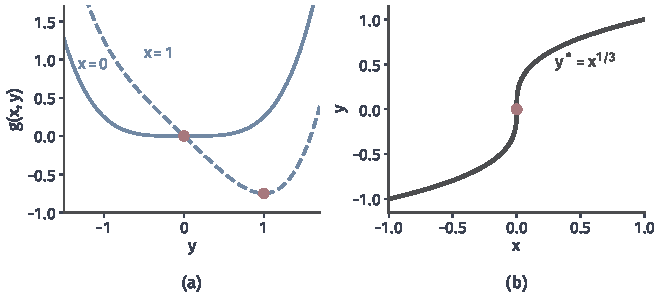
\includegraphics[width=112mm]{figures/05-optimization/07-multiple-criteria-and-nested-optimization/matplotlib/bilevel-singular/figure.pdf}
 \caption{内解唯一但不可微，$g=y^4/4-xy$。(a)$x=0$（实线）的碗底平坦，$H=0$；$x=1$（虚线）的碗底在$y=1$，红点是内解。(b)内解曲线$y^\star=x^{1/3}$连续，红点$x=0$处切线竖直。}
 \label{fig:bilevel-singular}
\end{BookInlineFigure}

\subsection{分支切换}
\label{sec:bilevel-switching}

内层非凸时，几个局部极小点可能并存，谁是全局最优随$\bm{x}$改变。局部分支一直光滑，全局选解却可能在某处跳到另一条分支上。

\paragraph{两个碗交换优劣}
构造一个可以手算的内层，它由两个抛物线取下包络：
\begin{equation}
 g(x,y)=\min\Bigl\{\frac12(y-1-x)^2-x,\ \ \frac12(y+1-x)^2+x\Bigr\}.
 \label{eq:bilevel-two-wells}
\end{equation}

令两式相等并化简，可知两条抛物线始终在$y=0$处相交，那里是两个碗之间的山脊。山脊不在碗底，所以每个碗底附近$g$就是一条光滑的抛物线，定理~\ref{thm:bilevel-local-branch}适用。第一个碗的碗底$y_+(x)=x+1$在$x>-1$时位于山脊右侧，第二个碗的碗底$y_-(x)=x-1$在$x<1$时位于山脊左侧。两个碗底的高度分别是
\[
 g(x,y_+(x))=-x,\qquad g(x,y_-(x))=x.
\]

所以$x>0$时右边的碗更低，$x<0$时左边的碗更低，$x=0$时打平。全局解集是
\[
 S(x)=\begin{cases}
 \{x-1\}, & x<0,\\
 \{-1,\ 1\}, & x=0,\\
 \{x+1\}, & x>0.
 \end{cases}
\]

图~\ref{fig:bilevel-switch-inner}(a)画了三个$x$处的$g$，(b)画了解曲线。全局选解在$x=0$处从下面一条分支跳到上面一条，两条分支本身都连续穿过$x=0$。

\begin{BookInlineFigure}
 \centering
 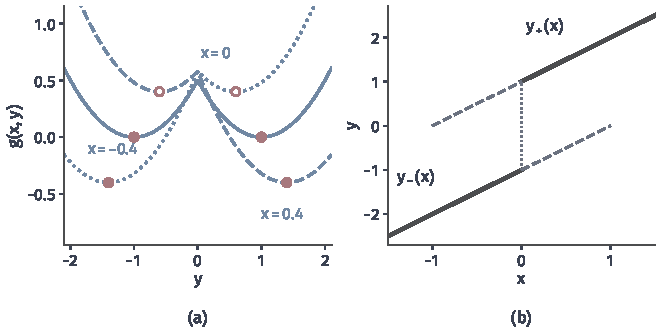
\includegraphics[width=112mm]{figures/05-optimization/07-multiple-criteria-and-nested-optimization/matplotlib/bilevel-switch-inner/figure.pdf}
 \caption{两个内层极小点交换优劣，$g$由式~\eqref{eq:bilevel-two-wells}定义。(a)$x=-0.4,0,0.4$时的$g$，红色实心点是全局极小点，空心点是非全局的局部极小点。(b)深灰粗线是全局内解，灰色虚线是仍为局部极小点、但已不是全局最优的分支延续，点线标出$x=0$处的跳变。}
 \label{fig:bilevel-switch-inner}
\end{BookInlineFigure}

\paragraph{外层目标跟着跳}
取外层目标$F=\frac12(y-\frac12)^2$。沿两条分支的外层值分别是
\[
 \Phi_+(x)=\frac12\Bigl(x+\frac12\Bigr)^2,\qquad\Phi_-(x)=\frac12\Bigl(x-\frac32\Bigr)^2.
\]

全局选解的外层值在$x>0$时是$\Phi_+$，在$x<0$时是$\Phi_-$。在$x=0$处从左极限$9/8$跳到右极限$1/8$，$\Phi$在这里甚至不连续。乐观模型在$x=0$选$y=1$，值为$1/8$；悲观模型选$y=-1$，值为$9/8$。

\paragraph{算法实际追踪的是哪一条}
现在假定外层用梯度下降，内层每次从上一轮的解继续求解。这种\term{热启动}（warm start）使内层一直留在右边的碗里。若沿分支用光滑公式，外层迭代是
\[
 x^{(t+1)}=x^{(t)}-\eta\,\Phi_+'(x^{(t)})=x^{(t)}-\eta\Bigl(x^{(t)}+\frac12\Bigr).
\]

从$x^{(0)}=0.8$出发，取$\eta=0.3$，迭代穿过$x=0$，一路收敛到$x=-\frac12$，此时外层值看上去是$0$。这是图~\ref{fig:bilevel-switch-phi}中的绿色路径。

可是$x=-\frac12$时右边的碗已经不是全局最优了。真正的内解在左边的碗里，$y_-(-\frac12)=-\frac32$，真实的外层值是
\[
 \Phi_-\Bigl(-\frac12\Bigr)=\frac12\Bigl(-\frac12-\frac32\Bigr)^2=2.
\]

算法报告的$0$和真实的$2$之间差了一条红色点线的距离，而算法运行中没有任何量发出警告，因为沿局部分支一切都光滑。

\begin{BookInlineFigure}
 \centering
 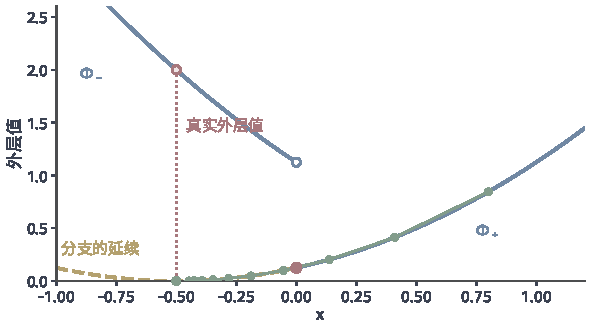
\includegraphics[width=100mm]{figures/05-optimization/07-multiple-criteria-and-nested-optimization/matplotlib/bilevel-switch-phi/figure.pdf}
 \caption{全局选解的外层值在切换点跳变，$F=\frac12(y-\frac12)^2$。蓝线是全局选解的外层值，$x=0$处的空心点是左极限$9/8$，红点是右极限$1/8$，也是乐观模型在$x=0$的值。黄色虚线是分支$\Phi_+$越过切换点后的延续，绿色路径是沿这条分支的外层梯度下降，它停在$x=-1/2$。红色空心点是此处真实的外层值$2$。}
 \label{fig:bilevel-switch-phi}
\end{BookInlineFigure}

表~\ref{tab:bilevel-three-derivatives}分清这里出现的三个“导数”。切换点处不能继续套用同一个光滑公式，这个公式求的是局部分支的导数，在切换点那一边它不再描述全局选解。

\begin{BookInlineTable}
 \centering
 \begin{tabular}{lll}
  \toprule
  对象 & 例中$x=-0.1$处 & 成立范围\\
  \midrule
  局部分支导数$\Phi_+'$ & $0.4$ & 分支存续的区间\\
  全局选解导数$\Phi_-'$ & $-1.6$ & 不含切换点的区间\\
  算法返回的导数 & 取决于碗的选择 & 取决于初值、热启动\\
  \bottomrule
 \end{tabular}
 \caption{分支切换时要区分的三种导数。例中$x=-0.1$时全局内解在左边的碗，热启动的算法却可能仍在右边的碗。}
 \label{tab:bilevel-three-derivatives}
\end{BookInlineTable}

\section{隐式微分}
\label{sec:bilevel-implicit}

在定理~\ref{thm:bilevel-local-branch}成立的分支上，怎样计算外层目标的导数？关键的观察是，求导只需要当前解点处的局部关系。至于这个解是怎样迭代得到的，算法走过了多少步，都不进入公式，也不必保存。

\subsection{超梯度}
\label{sec:bilevel-hypergradient}

设$\hat{\bm{y}}(\bm{x})$是所追踪的分支，外层目标为$\Phi(\bm{x})=F(\bm{x},\hat{\bm{y}}(\bm{x}))$。若内解唯一且满足定理~\ref{thm:bilevel-strong-convex-map}，这条分支就是$\bm{y}^\star(\bm{x})$。$\Phi$对$\bm{x}$的梯度称为\termalias{超梯度-hypergradient}{超梯度}（hypergradient）。“超”在这里指外层，与第~\ref{chap:penalty-multiplier-methods}章凹函数的超梯度（supergradient）是两回事。

\paragraph{主要思想：把响应接到外层}
由链式法则，$\Phi$的梯度由两部分组成：
\[
 \nabla\Phi=\nabla_{\bm{x}}F+\bm{D}^{\top}\nabla_{\bm{y}}F.
\]
第一项是直接作用，第二项是响应。把式~\eqref{eq:bilevel-branch-derivative}代入第二项，并利用$\bm{H}$对称，得到
\[
 \bm{D}^{\top}\nabla_{\bm{y}}F=-\bm{B}^{\top}\bm{H}^{-1}\nabla_{\bm{y}}F.
\]

这个式子不必先算出$\bm{H}^{-1}\bm{B}$这个$d\times n$矩阵。先解一个以$\nabla_{\bm{y}}F$为右端的方程，得到的向量再乘$\bm{B}^{\top}$即可。

\begin{theorem}[隐式超梯度]
\label{thm:bilevel-hypergradient}
设定理~\ref{thm:bilevel-local-branch}的条件成立，$F$在$(\bm{x}_0,\bm{y}_0)$附近连续可微。则$\Phi(\bm{x})=F(\bm{x},\hat{\bm{y}}(\bm{x}))$连续可微，且
\begin{equation}
 \nabla\Phi=\nabla_{\bm{x}}F-\bm{B}^{\top}\bm{v},
 \qquad\bm{H}\bm{v}=\nabla_{\bm{y}}F,
 \label{eq:bilevel-hypergradient}
\end{equation}
其中所有导数都在$(\bm{x},\hat{\bm{y}}(\bm{x}))$处取值。
\end{theorem}

\begin{proof}
$\hat{\bm{y}}$连续可微，$F$连续可微，由链式法则$\Phi$连续可微，其梯度是上面的两项之和。$\bm{H}$正定，所以方程$\bm{H}\bm{v}=\nabla_{\bm{y}}F$有唯一解，即$\bm{v}=\bm{H}^{-1}\nabla_{\bm{y}}F$，代入即得式~\eqref{eq:bilevel-hypergradient}。
\end{proof}

式~\eqref{eq:bilevel-hypergradient}中的$\bm{H}\bm{v}=\nabla_{\bm{y}}F$称为\term{伴随方程}（adjoint equation）。用这种方法求超梯度的做法称为\term{隐式微分}（implicit differentiation），因为内解没有显式公式，导数是从定义它的方程中得出的。

\paragraph{$\bm{v}$是内层梯度的价格}
$\bm{v}$有一个直接的含义。设想把驻点方程改成$\nabla_{\bm{y}}g=\bm{\varepsilon}$，也就是给内层梯度一点小扰动。内解移动$\bm{H}^{-1}\bm{\varepsilon}$，外层值变化约为
\[
 \langle\nabla_{\bm{y}}F,\bm{H}^{-1}\bm{\varepsilon}\rangle=\langle\bm{v},\bm{\varepsilon}\rangle.
\]
所以$\bm{v}$是内层梯度每单位扰动在外层的价格，含义和约束乘子作为影子价格相同。

$\bm{x}$改变$\Delta\bm{x}$时，内层梯度在原来的解点偏移$\bm{B}\Delta\bm{x}$，内解要把这份偏移抵消掉，相当于对内层施加了$-\bm{B}\Delta\bm{x}$的扰动。价格乘以扰动量，就得到响应项$-\langle\bm{B}^{\top}\bm{v},\Delta\bm{x}\rangle$。这个价格只在一阶范围内有效，$\Delta\bm{x}$大了或分支切换了，它就不再准确。

图~\ref{fig:bilevel-adjoint-chain}把这条因果链画了出来。上面一行顺着原因往下算，要带着$n$个方向的$\Delta\bm{x}$走完全程。下面一行从外层往回算，只带一个向量。标量外层目标、很多外层变量时，后者便宜得多。

\begin{BookInlineFigure}
 \centering
 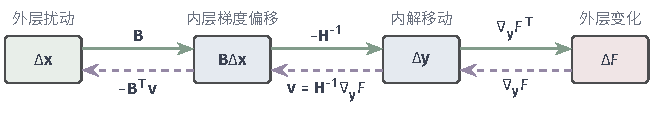
\includegraphics[width=110.6mm]{figures/05-optimization/07-multiple-criteria-and-nested-optimization/tikz/bilevel-adjoint-chain/figure.pdf}
 \caption{超梯度的因果链。绿色实线从外层扰动算到外层变化，每个方向$\Delta\bm{x}$算一次。紫色虚线从外层梯度往回算，一次得到全部分量的梯度，$\bm{v}$是内层梯度偏移的价格。}
 \label{fig:bilevel-adjoint-chain}
\end{BookInlineFigure}

\paragraph{手算核对}
对正则拟合例~\eqref{eq:bilevel-ridge}，在$x=1$处，各量为
\[
 y^\star=\frac32,\qquad H=1+x=2,\qquad B=y^\star=\frac32,\qquad\partial_yF=y^\star-1=\frac12.
\]

解伴随方程，得到
\[
 v=\frac{\partial_yF}{H}=\frac14.
\]

$F$不含$x$，所以由式~\eqref{eq:bilevel-hypergradient}，
\[
 \Phi'(1)=0-Bv=-\frac38.
\]

直接对$\Phi$求导来核对。由链式法则，
\[
 \Phi'(x)=(y^\star-1)\,\frac{\mathrm{d}y^\star}{\mathrm{d}x},
\]
在$x=1$处等于$\frac12\times(-\frac34)=-\frac38$，两者相同。同样可算出$\Phi'(0)=-6$；在$x=2$处$\partial_yF=0$，$v=0$，$\Phi'(2)=0$，这正是最小点。

\paragraph{第二项不能丢}
这个例子里$\nabla_{\bm{x}}F=0$。如果只对$F$求偏导，也就是把$y$固定住，得到的斜率处处是$0$，结论将是$x$不用调整。图~\ref{fig:bilevel-hypergrad-tangent}比较了这两条线。忽略响应项，求的是“固定内解时的偏导数”，并不是双层目标的导数。

\begin{BookInlineFigure}
 \centering
 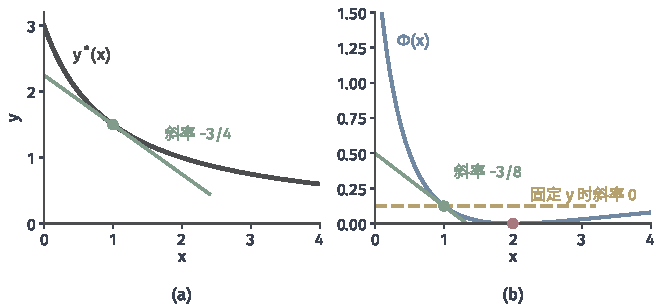
\includegraphics[width=112mm]{figures/05-optimization/07-multiple-criteria-and-nested-optimization/matplotlib/bilevel-hypergrad-tangent/figure.pdf}
 \caption{正则拟合例中$x=1$处的导数。(a)内解曲线的切线，斜率是$\mathrm{d}y^\star/\mathrm{d}x=-3/4$。(b)$\Phi$的切线（绿）斜率是超梯度$-3/8$；黄色虚线是把$y$固定在$y^\star(1)$时的外层函数，斜率为$0$。红点是$\Phi$的最小点。}
 \label{fig:bilevel-hypergrad-tangent}
\end{BookInlineFigure}

\paragraph{与极小极大的联系}
式~\eqref{eq:bilevel-hypergradient}也说明了表~\ref{tab:bilevel-vs-minimax}的最后一行。若$F=-g$，内解处$\nabla_{\bm{y}}F=-\nabla_{\bm{y}}g=\bm{0}$，于是$\bm{v}=\bm{0}$，超梯度退化为$\nabla_{\bm{x}}F$。内解的移动对外层值只有二阶影响，这就是第~\ref{chap:minimax-optimization}章和第~\ref{chap:parametric-sensitivity}章的包络关系。一般的双层问题没有这种抵消，响应项必须计算。

\subsection{线性方程求解}
\label{sec:bilevel-linear-solve}

$d$很大时$\bm{H}$存不下，更不用说求逆。本小节要解决的问题是：怎样只用$\bm{H}$与向量的乘积解伴随方程，以及这个方程解得不准会造成多大的超梯度误差。

\paragraph{主要思想：只用矩阵—向量积}
解$\bm{H}\bm{v}=\nabla_{\bm{y}}F$的迭代法只需要反复计算$\bm{H}\bm{u}$。这个乘积不需要$\bm{H}$的元素，它是内层梯度沿$\bm{u}$方向的方向导数：
\begin{equation}
 \bm{H}\bm{u}=\frac{\mathrm{d}}{\mathrm{d}s}\nabla_{\bm{y}}g(\bm{x},\bm{y}+s\bm{u})\Big|_{s=0}.
 \label{eq:bilevel-hvp}
\end{equation}

这称为\term{Hessian向量积}（Hessian-vector product）。用自动求导时，它的代价是梯度计算的常数倍，也可以用内层梯度的差分近似。$\bm{B}^{\top}\bm{v}$同样如此，它是标量$\langle\nabla_{\bm{y}}g,\bm{v}\rangle$（固定$\bm{v}$）对$\bm{x}$的梯度。

$\bm{H}$对称正定时，共轭梯度法是自然的选择，算法的推导可参考\BookChapterRef{chap:krylov-methods}{卷二第15章“Krylov子空间法”}。第~$k$步用到的量都按下面的递推得到，$\alpha^{(k)}$和$\beta^{(k)}$在本小节里表示共轭梯度法自己的系数：
\begin{equation}
 \begin{gathered}
 \alpha^{(k)}=\frac{\lVert\bm{r}^{(k)}\rVert_2^2}{\langle\bm{d}^{(k)},\bm{H}\bm{d}^{(k)}\rangle},\qquad
 \bm{v}^{(k+1)}=\bm{v}^{(k)}+\alpha^{(k)}\bm{d}^{(k)},\\
 \bm{r}^{(k+1)}=\bm{r}^{(k)}-\alpha^{(k)}\bm{H}\bm{d}^{(k)},\\
 \beta^{(k)}=\frac{\lVert\bm{r}^{(k+1)}\rVert_2^2}{\lVert\bm{r}^{(k)}\rVert_2^2},\qquad
 \bm{d}^{(k+1)}=\bm{r}^{(k+1)}+\beta^{(k)}\bm{d}^{(k)}.
 \end{gathered}
 \label{eq:bilevel-cg}
\end{equation}

\paragraph{计算过程}
下面用二维内层走一遍全过程。内层是带二次惩罚的最小二乘，外层把结果和目标点比较：
\[
 g(x,\bm{y})=\frac12\lVert\bm{A}\bm{y}-\bm{b}\rVert_2^2+\frac{x}{2}\lVert\bm{y}\rVert_2^2,\qquad F(\bm{y})=\frac12\lVert\bm{y}-\bm{c}\rVert_2^2.
\]

数据取为
\[
 \bm{A}=\begin{bmatrix}1&1\\0&1\end{bmatrix},\qquad
 \bm{b}=\begin{bmatrix}3\\1\end{bmatrix},\qquad
 \bm{c}=\begin{bmatrix}0\\2\end{bmatrix}.
\]

\needspace{6\baselineskip}
\paragraph{变量}
\begin{itemize}
 \item 内解$\bm{y}\in\mathbb{R}^d$，事先由内层算法得到。
 \item 伴随向量的迭代值$\bm{v}^{(k)}\in\mathbb{R}^d$，残差$\bm{r}^{(k)}=\nabla_{\bm{y}}F-\bm{H}\bm{v}^{(k)}$，搜索方向$\bm{d}^{(k)}\in\mathbb{R}^d$。
 \item 超梯度估计$\hat{\bm{\gamma}}^{(k)}\in\mathbb{R}^n$，把式~\eqref{eq:bilevel-hypergradient}中的$\bm{v}$换成$\bm{v}^{(k)}$得到。
\end{itemize}

\paragraph{初始化}
先在当前$\bm{x}$处得到内解，计算外层梯度，并置$\bm{v}^{(0)}=\bm{0}$，$\bm{r}^{(0)}=\bm{d}^{(0)}=\nabla_{\bm{y}}F$。

例中取$x=1$。$\bm{H}=\bm{A}^{\top}\bm{A}+x\bm{I}$，解$\bm{H}\bm{y}=\bm{A}^{\top}\bm{b}$得到内解，于是
\[
 \bm{H}=\begin{bmatrix}2&1\\1&3\end{bmatrix},\qquad
 \bm{y}=\begin{bmatrix}1\\1\end{bmatrix},\qquad
 \bm{r}^{(0)}=\bm{y}-\bm{c}=\begin{bmatrix}1\\-1\end{bmatrix}.
\]
$\bm{H}$的两个特征值都为正，共轭梯度法适用。内层梯度对$x$的导数是$\bm{y}$，所以$\bm{B}=\bm{y}$，$\nabla_xF=0$。

\needspace{6\baselineskip}
\paragraph{每轮更新}
\begin{enumerate}
 \item 计算$\bm{H}\bm{d}^{(k)}$，按式~\eqref{eq:bilevel-cg}得到$\alpha^{(k)}$，更新$\bm{v}$和$\bm{r}$。

 例中第一轮，$\bm{H}\bm{d}^{(0)}=(1,-2)$，于是
 \[
  \alpha^{(0)}=\frac{2}{3},\qquad
  \bm{v}^{(1)}=\frac23\begin{bmatrix}1\\-1\end{bmatrix},\qquad
  \bm{r}^{(1)}=\frac13\begin{bmatrix}1\\1\end{bmatrix}.
 \]
 此时的超梯度估计是$-\bm{y}^{\top}\bm{v}^{(1)}=0$。

 \item 按式~\eqref{eq:bilevel-cg}计算$\beta^{(k)}$，更新搜索方向。

 例中第一轮，
 \[
  \beta^{(0)}=\frac{2/9}{2}=\frac19,\qquad
  \bm{d}^{(1)}=\frac13\begin{bmatrix}1\\1\end{bmatrix}+\frac19\begin{bmatrix}1\\-1\end{bmatrix}=\frac29\begin{bmatrix}2\\1\end{bmatrix}.
 \]

 例中第二轮，先算矩阵—向量积和分母：
 \[
  \bm{H}\bm{d}^{(1)}=\frac{10}{9}\begin{bmatrix}1\\1\end{bmatrix},\qquad\langle\bm{d}^{(1)},\bm{H}\bm{d}^{(1)}\rangle=\frac{20}{27}.
 \]
 于是
 \[
  \alpha^{(1)}=\frac{2/9}{20/27}=\frac{3}{10},\qquad
  \bm{v}^{(2)}=\frac15\begin{bmatrix}4\\-3\end{bmatrix},\qquad
  \bm{r}^{(2)}=\bm{0}.
 \]

 \item 残差范数低于设定精度时停止，否则回到第1步。例中$\bm{r}^{(2)}=\bm{0}$，两步结束。
\end{enumerate}

最终得到$\bm{v}=(4/5,-3/5)$，由式~\eqref{eq:bilevel-hypergradient}，超梯度是
\[
 \Phi'(1)=-\bm{y}^{\top}\bm{v}=-\frac15.
\]

直接验证。由式~\eqref{eq:bilevel-branch-derivative}，内解的导数是
\[
 \frac{\mathrm{d}\bm{y}}{\mathrm{d}x}=-\bm{H}^{-1}\bm{y}=-\frac15\begin{bmatrix}2\\1\end{bmatrix},
\]
它与$\nabla_{\bm{y}}F=(1,-1)$的内积是$-1/5$，结果一致。第一轮的残差非零，超梯度估计是$0$，没有反映出真实的下降方向。这引出了下面的误差分析。

\paragraph{共轭梯度法的前提}
式~\eqref{eq:bilevel-cg}的分母要求$\langle\bm{d},\bm{H}\bm{d}\rangle>0$，这需要$\bm{H}$正定。在局部极小点的分支上这成立，但内层非凸且当前点还没收敛时可能不成立。取$\bm{H}=\operatorname{diag}(1,-1)$，$\bm{r}^{(0)}=(1,1)$，第一步的分母就是$1-1=0$，算法无法进行。这时应先检查所在位置是否还在所说的分支上，再选择适用于不定矩阵的求解方法。

\paragraph{线性残差怎样变成超梯度误差}
设$\tilde{\bm{v}}$是近似解，残差$\bm{r}=\bm{H}\tilde{\bm{v}}-\nabla_{\bm{y}}F$。线性方程的残差很小，并不等于超梯度的误差很小，中间隔着$\bm{H}^{-1}$和$\bm{B}$。

\begin{theorem}[伴随残差的放大]
\label{thm:bilevel-residual-amplification}
设内解精确，$\bm{H}\succeq\mu\bm{I}$，$\tilde{\bm{\gamma}}$是把式~\eqref{eq:bilevel-hypergradient}中的$\bm{v}$换成$\tilde{\bm{v}}$所得的估计，残差$\bm{r}=\bm{H}\tilde{\bm{v}}-\nabla_{\bm{y}}F$。则
\begin{equation}
 \lVert\tilde{\bm{\gamma}}-\nabla\Phi\rVert_2\leq\frac{\lVert\bm{B}\rVert_2}{\mu}\,\lVert\bm{r}\rVert_2.
 \label{eq:bilevel-residual-amplification}
\end{equation}
\end{theorem}

\begin{proof}
由残差的定义，$\tilde{\bm{v}}-\bm{v}=\bm{H}^{-1}\bm{r}$，所以
\[
 \tilde{\bm{\gamma}}-\nabla\Phi=-\bm{B}^{\top}(\tilde{\bm{v}}-\bm{v})=-\bm{B}^{\top}\bm{H}^{-1}\bm{r}.
\]
再用$\lVert\bm{H}^{-1}\rVert_2\leq1/\mu$取范数即得。
\end{proof}

上面例子的第一轮，$\lVert\bm{r}^{(1)}\rVert_2=\sqrt{2}/3\approx0.471$，$\lVert\bm{B}\rVert_2=\sqrt2$，$\bm{H}$的最小特征值是$(5-\sqrt5)/2\approx1.382$。代入式~\eqref{eq:bilevel-residual-amplification}，上界约为$0.482$，实际误差是$0.2$。

式~\eqref{eq:bilevel-residual-amplification}说明，内层越病态，同样的残差放大得越厉害；而且病态也让共轭梯度法收敛更慢。图~\ref{fig:bilevel-cg}中，$\kappa=10$时残差很快下降，超梯度误差跟着下降；$\kappa=1000$时残差下降缓慢，超梯度误差还比残差大几倍到几十倍。内层病态的问题需要把线性方程解得更准，这笔账要算进总成本。

\begin{BookInlineFigure}
 \centering
 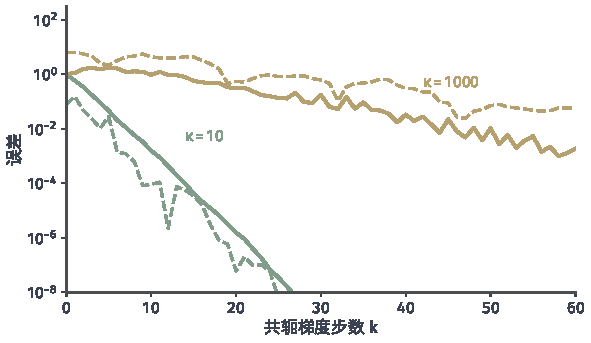
\includegraphics[width=100mm]{figures/05-optimization/07-multiple-criteria-and-nested-optimization/matplotlib/bilevel-cg/figure.pdf}
 \caption{共轭梯度法解伴随方程的收敛，$d=60$，$\bm{H}$的特征值在$[1/\kappa,1]$上对数均匀分布，$\bm{B}$、$\nabla_{\bm{y}}F$是固定种子下的随机单位向量。实线是残差范数，虚线是超梯度的绝对误差。绿色$\kappa=10$，黄色$\kappa=1000$。}
 \label{fig:bilevel-cg}
\end{BookInlineFigure}

\paragraph{另一种近似：Neumann级数}
若$0<\alpha<2/\lambda_{\max}(\bm{H})$，矩阵$\bm{I}-\alpha\bm{H}$的谱半径小于$1$，$\bm{H}^{-1}$可以展开为级数：
\begin{equation}
 \bm{H}^{-1}=\alpha\sum_{k=0}^{\infty}(\bm{I}-\alpha\bm{H})^k.
 \label{eq:bilevel-neumann}
\end{equation}
只取前$\ell$项，就得到一种只用Hessian向量积的近似。它收敛比共轭梯度法慢，但第~\ref{sec:bilevel-truncated}小节会看到，它恰好就是截断展开的极限形式。

\subsection{约束内层}
\label{sec:bilevel-constrained-inner}

内层有约束时，内解满足的不再是驻点方程，$\bm{H}$的位置也要换成整个KKT系统。本小节要解决的问题是：什么时候这样做是对的，以及哪些情况下根本不存在经典的导数。

\paragraph{主要思想：对活动的KKT方程求导}
$g$已用作内层目标，这里把内层约束写成$c_i(\bm{x},\bm{y})\leq0$（$i=1,\ldots,m$）和$h_j(\bm{x},\bm{y})=0$（$j=1,\ldots,p$），Lagrange函数是
\begin{equation}
 \mathcal{L}(\bm{x},\bm{y},\bm{\lambda},\bm{\nu})=g+\sum_{i=1}^{m}\lambda_ic_i+\sum_{j=1}^{p}\nu_jh_j.
 \label{eq:bilevel-lagrangian}
\end{equation}

第~\ref{chap:constrained-optimality}章的KKT条件和第~\ref{chap:parametric-sensitivity}章的敏感性定理告诉我们：在基准KKT点处，若线性无关约束资格（LICQ）、严格互补和二阶充分条件成立，则存在邻域内的连续可微分支，活动集$A$在分支上保持不变，分支上的点都是严格局部极小点。

把活动不等式当成等式，记活动不等式与等式的总数为$a+p$，定义四个矩阵。前两个是$\mathcal{L}$的二阶导数：
\[
 \bm{W}=\nabla^2_{\bm{y}\bm{y}}\mathcal{L},\qquad\bm{B}_{\mathcal{L}}=\nabla^2_{\bm{y}\bm{x}}\mathcal{L}.
\]
另外两个来自约束：$\bm{J}$的行是活动约束和等式约束对$\bm{y}$的梯度，$\bm{E}$的行是它们对$\bm{x}$的梯度。KKT矩阵为
\begin{equation}
 \bm{K}=\begin{bmatrix}\bm{W}&\bm{J}^{\top}\\\bm{J}&\bm{0}\end{bmatrix}.
 \label{eq:bilevel-kkt-matrix}
\end{equation}

\begin{theorem}[约束内层的隐式超梯度]
\label{thm:bilevel-constrained-hypergradient}
设在基准KKT点处$g,c_i,h_j$二阶连续可微，LICQ、严格互补与二阶充分条件成立，$F$连续可微。则$\Phi(\bm{x})=F(\bm{x},\hat{\bm{y}}(\bm{x}))$在基准点附近连续可微，且
\begin{equation}
 \nabla\Phi=\nabla_{\bm{x}}F-\bm{B}_{\mathcal{L}}^{\top}\bm{v}-\bm{E}^{\top}\bm{w},
 \qquad
 \bm{K}\begin{bmatrix}\bm{v}\\\bm{w}\end{bmatrix}=\begin{bmatrix}\nabla_{\bm{y}}F\\\bm{0}\end{bmatrix}.
 \label{eq:bilevel-constrained-hypergradient}
\end{equation}
\end{theorem}

\begin{proof}
由第~\ref{chap:parametric-sensitivity}章的不等式约束解导数定理，$\bm{K}$可逆，分支的Jacobian矩阵$\bm{D}$与乘子导数$\bm{D}_{\bm{w}}$满足
\[
 \bm{K}\begin{bmatrix}\bm{D}\\\bm{D}_{\bm{w}}\end{bmatrix}=-\begin{bmatrix}\bm{B}_{\mathcal{L}}\\\bm{E}\end{bmatrix}.
\]

取$(\bm{v},\bm{w})$为式~\eqref{eq:bilevel-constrained-hypergradient}中方程的解，并用$\bm{K}$对称，得到
\[
 \bm{D}^{\top}\nabla_{\bm{y}}F=\begin{bmatrix}\bm{D}\\\bm{D}_{\bm{w}}\end{bmatrix}^{\top}\bm{K}\begin{bmatrix}\bm{v}\\\bm{w}\end{bmatrix}=-\bm{B}_{\mathcal{L}}^{\top}\bm{v}-\bm{E}^{\top}\bm{w}.
\]
代入第~\ref{sec:bilevel-hypergradient}小节开头的链式法则即得。
\end{proof}

\paragraph{预算例}
外层变量取预算$x=\tau$，内层沿用第~\ref{chap:parametric-sensitivity}章的预算二次问题的主要部分，外层想让配置接近另一个点：
\[
 \begin{aligned}
 g(\bm{y})&=\frac12(y_1-2)^2+\frac12(y_2-1)^2,\quad c(\tau,\bm{y})=y_1+y_2-\tau\leq0,\\
 F(\bm{y})&=\frac12(y_1-2)^2+\frac12(y_2-2)^2.
 \end{aligned}
\]

在$\tau=2$处约束活动，内解和乘子是$\bm{y}=(3/2,1/2)$，$\lambda=1/2>0$，严格互补成立。各块矩阵和右端为
\[
 \bm{W}=\bm{I},\quad\bm{J}=\begin{bmatrix}1&1\end{bmatrix},\quad\bm{B}_{\mathcal{L}}=\bm{0},\quad E=-1,\quad\nabla_{\bm{y}}F=\begin{bmatrix}-1/2\\-3/2\end{bmatrix}.
\]

式~\eqref{eq:bilevel-constrained-hypergradient}的方程组写开是
\[
 v_1+w=-\frac12,\qquad v_2+w=-\frac32,\qquad v_1+v_2=0.
\]

前两式相加并用第三式，得$w=-1$，于是$v_1=1/2$，$v_2=-1/2$。代入超梯度公式，
\[
 \Phi'(2)=-E\,w=-1.
\]

直接核对：约束活动时$\bm{y}=((1+\tau)/2,(\tau-1)/2)$，它对$\tau$的导数是$(1/2,1/2)$，与$\nabla_{\bm{y}}F$的内积是$-1$。图~\ref{fig:bilevel-kkt-kink}(a)的绿线是这条解路径。

\paragraph{公式失效的情形}
活动集变化时导数会断。预算例中$\lambda=(3-\tau)/2$，到$\tau=3$时乘子降为零，严格互补失效，内解停在理想点$(2,1)$。外层值的左导数由$(\tau-4)/2$给出，在$\tau=3$处等于$-1/2$；$\tau>3$时外层值是常数，右导数是$0$。这就是图~\ref{fig:bilevel-kkt-kink}(b)的折点，经典的导数在此不存在。

\begin{BookInlineFigure}
 \centering
 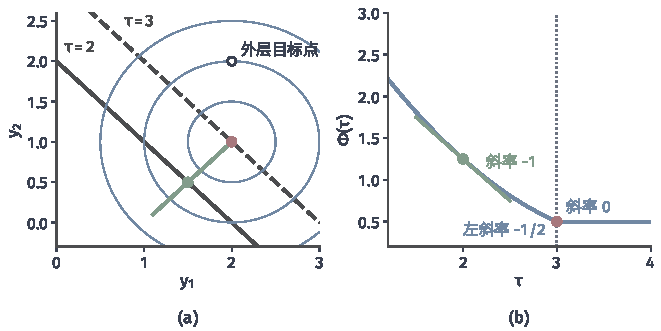
\includegraphics[width=112mm]{figures/05-optimization/07-multiple-criteria-and-nested-optimization/matplotlib/bilevel-kkt-kink/figure.pdf}
 \caption{约束内层的预算例。(a)蓝色等高线属于内层目标，红点是无约束最优$(2,1)$，深灰实线和虚线分别是$\tau=2$和$\tau=3$的预算线，绿线是内解随$\tau$移动的路径，绿点是$\tau=2$的解，空心点是外层目标点$(2,2)$。(b)外层值$\Phi(\tau)$，绿色切线在$\tau=2$处斜率$-1$；红点$\tau=3$处活动集改变，左斜率$-1/2$，右斜率$0$。}
 \label{fig:bilevel-kkt-kink}
\end{BookInlineFigure}

$\bm{K}$奇异时公式不能使用，但内解不一定不可微。取内层$\min\frac12(y-2)^2$，约束$y\leq\tau$和$2y\leq2\tau$是同一条约束的两种写法。在$\tau=1$处两者都活动，$\bm{J}$的两行成比例，LICQ失效，$\bm{K}$奇异，乘子也不唯一。而内解$y=\min\{\tau,2\}$在$\tau=1$附近的导数是$1$，完全正常。

还有一种常见的错误，是把$\bm{H}$换成$\bm{W}$，仍用式~\eqref{eq:bilevel-hypergradient}。预算例中$\bm{W}=\bm{I}$，$\bm{B}_{\mathcal{L}}=\bm{0}$，这样算出的解导数是零向量，而真实导数是$(1/2,1/2)$。约束的作用全在$\bm{J}$和$\bm{E}$里，只换一个矩阵等于把约束的响应丢掉了。

\section{迭代展开}
\label{sec:bilevel-unrolling}

隐式微分依赖“内层已经到了解点”这一前提。如果真正运行的是有限步算法，也可以直接对算法的输出求导。于是要问：怎样对$\bm{y}^{(T)}(\bm{x})$求导，这样算出的量和隐式导数有什么关系？这种做法称为\term{迭代展开}（unrolled differentiation）。

设内层的一步更新写成
\begin{equation}
 \bm{y}^{(t+1)}=\bm{\Psi}_t(\bm{y}^{(t)},\bm{x}),\qquad t=0,\ldots,T-1.
 \label{eq:bilevel-update}
\end{equation}
梯度下降取$\bm{\Psi}_t=\bm{y}-\alpha\nabla_{\bm{y}}g$，这些更新规则本身的性质在第~\ref{chap:first-order-methods}章讨论，下面只处理沿更新传播导数时新增的对象。

\subsection{完整展开}
\label{sec:bilevel-full-unroll}

\paragraph{主要思想：把算法看成复合函数}
$\bm{y}^{(T)}$是$\bm{x}$经过$T$层复合得到的函数，对它求导只需要反复使用链式法则。图~\ref{fig:bilevel-unroll-graph}是$T=2$的计算图，$\bm{x}$进入每一步更新，所以每一层都要算一次它的影响。

\begin{BookInlineFigure}
 \centering
 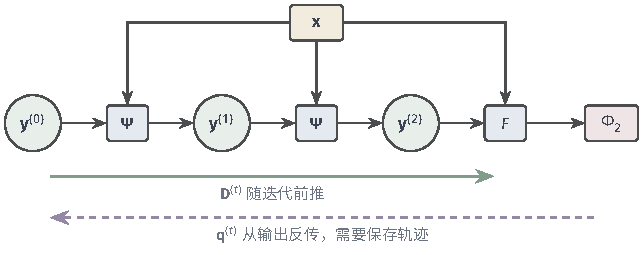
\includegraphics[width=108.9mm]{figures/05-optimization/07-multiple-criteria-and-nested-optimization/tikz/bilevel-unroll-graph/figure.pdf}
 \caption{$T=2$时的展开计算图。圆圈是内层状态，方框$\bm{\Psi}$是一步更新，$\bm{x}$进入每步更新和外层目标。绿色实线表示前向传播Jacobian矩阵$\bm{D}^{(t)}$，紫色虚线表示从外层往回传播向量$\bm{q}^{(t)}$。}
 \label{fig:bilevel-unroll-graph}
\end{BookInlineFigure}

记$\bm{D}^{(t)}\in\mathbb{R}^{d\times n}$为$\bm{y}^{(t)}$对$\bm{x}$的Jacobian矩阵，并记一步更新的两个偏导数：
\[
 \bm{A}^{(t)}=\frac{\partial\bm{\Psi}_t}{\partial\bm{y}}\in\mathbb{R}^{d\times d},\qquad
 \bm{C}^{(t)}=\frac{\partial\bm{\Psi}_t}{\partial\bm{x}}\in\mathbb{R}^{d\times n}.
\]
两者都在$(\bm{y}^{(t)},\bm{x})$处取值。对梯度下降，$\bm{A}^{(t)}=\bm{I}-\alpha\bm{H}^{(t)}$，$\bm{C}^{(t)}=-\alpha\bm{B}^{(t)}$，其中$\bm{H}^{(t)}$、$\bm{B}^{(t)}$是在当前迭代点算出的二阶导数。

对式~\eqref{eq:bilevel-update}两边关于$\bm{x}$求导。$\bm{y}^{(t)}$本身依赖$\bm{x}$，所以
\begin{equation}
 \bm{D}^{(t+1)}=\bm{A}^{(t)}\bm{D}^{(t)}+\bm{C}^{(t)}.
 \label{eq:bilevel-forward}
\end{equation}

有限步目标的梯度由链式法则得到：
\begin{equation}
 \nabla\Phi_T=\nabla_{\bm{x}}F+(\bm{D}^{(T)})^{\top}\nabla_{\bm{y}}F,
 \label{eq:bilevel-finite-gradient}
\end{equation}
其中$F$的导数在$(\bm{x},\bm{y}^{(T)})$处取值。这是精确的导数，只不过它是$\Phi_T$的导数。

\paragraph{主要思想：反向累积}
式~\eqref{eq:bilevel-forward}要带着一个$d\times n$矩阵走完全程，$n$很大时存不下。把递推展开，得到
\[
 \bm{D}^{(T)}=\sum_{t=0}^{T-1}\bm{A}^{(T-1)}\cdots\bm{A}^{(t+1)}\bm{C}^{(t)}+\bm{A}^{(T-1)}\cdots\bm{A}^{(0)}\bm{D}^{(0)}.
\]

式~\eqref{eq:bilevel-finite-gradient}只需要这个矩阵的转置与一个向量的乘积，可以从左边的向量开始依次向右乘。令$\bm{q}^{(T)}=\nabla_{\bm{y}}F$，从$t=T-1$到$0$计算
\begin{equation}
 \bm{h}\leftarrow\bm{h}+(\bm{C}^{(t)})^{\top}\bm{q}^{(t+1)},\qquad
 \bm{q}^{(t)}=(\bm{A}^{(t)})^{\top}\bm{q}^{(t+1)}.
 \label{eq:bilevel-reverse}
\end{equation}
$\bm{h}$的初值是$\nabla_{\bm{x}}F$，循环结束后再加上$(\bm{D}^{(0)})^{\top}\bm{q}^{(0)}$，结果就是$\nabla\Phi_T$。

两种顺序保存的东西不同。前向传播保存$\bm{D}^{(t)}$，不用保存轨迹。反向累积只保存向量，但$\bm{A}^{(t)}$、$\bm{C}^{(t)}$要在$\bm{y}^{(t)}$处计算，所以必须把整条轨迹保存下来，或者重新算出来。

\paragraph{计算过程}
用正则拟合例在$x=0$处计算$\Phi_3'(0)$，内层取$y^{(0)}=0$，$\alpha=1/2$。

\needspace{6\baselineskip}
\paragraph{变量}
\begin{itemize}
 \item 迭代点$y^{(t)}$，前向时的导数$D^{(t)}$，这里$d=n=1$，它们都是数。
 \item 一步更新的偏导数$A^{(t)}=1-\alpha(1+x)$，$C^{(t)}=-\alpha y^{(t)}$。
 \item 反向时的累积量$q^{(t)}$和结果$h$。
\end{itemize}

\paragraph{初始化}
初值不依赖$x$，所以$D^{(0)}=0$。例中$x=0$，于是$A^{(t)}=1/2$，$C^{(t)}=-y^{(t)}/2$。

\needspace{6\baselineskip}
\paragraph{每轮更新}
\begin{enumerate}
 \item 前向：更新$y^{(t+1)}$，并按式~\eqref{eq:bilevel-forward}更新$D^{(t+1)}$。

 例中第一轮$D^{(1)}=\frac12\cdot0-\frac12\cdot0=0$，第二轮用$y^{(1)}=3/2$，第三轮用$y^{(2)}=9/4$，各轮结果为
 \[
  y^{(1)},y^{(2)},y^{(3)}=\frac32,\ \frac94,\ \frac{21}{8};\qquad
  D^{(1)},D^{(2)},D^{(3)}=0,\ -\frac34,\ -\frac32.
 \]

 \item 走完$T$步后由式~\eqref{eq:bilevel-finite-gradient}得到梯度。

 例中$\partial_yF=y^{(3)}-1=13/8$，$\partial_xF=0$，于是
 \[
  \Phi_3'(0)=D^{(3)}\cdot\frac{13}{8}=-\frac{39}{16}.
 \]

 \item 反向：若改用反向累积，从$q^{(3)}=13/8$、$h=0$开始按式~\eqref{eq:bilevel-reverse}回算。

 例中$t=2$时$C^{(2)}=-9/8$，$t=1$时$C^{(1)}=-3/4$，$t=0$时$C^{(0)}=0$，各轮结果为
 \[
  h:\ -\frac{117}{64},\ -\frac{156}{64},\ -\frac{156}{64};\qquad
  q^{(2)},q^{(1)},q^{(0)}=\frac{13}{16},\ \frac{13}{32},\ \frac{13}{64}.
 \]
\end{enumerate}

最终$h=-156/64=-39/16$，与前向结果相同。这个数是$\Phi_3$的精确导数，而$\Phi$的导数是$-6$，两者相差很大，都是正确的导数，只是对应不同的目标。

\paragraph{初始化、动量与不可微更新}
若初值依赖$\bm{x}$，$\bm{D}^{(0)}$不为零，它的贡献必须保留。用上一轮解作热启动时，严格说初值也依赖过去的$\bm{x}$，把这一项丢掉就是在计算另一个量的导数。

算法含动量时，一步更新依赖不止一个迭代点。例如重球法的更新是
\[
 \bm{y}^{(t+1)}=\bm{y}^{(t)}-\alpha\nabla_{\bm{y}}g+\omega(\bm{y}^{(t)}-\bm{y}^{(t-1)}),
\]
要把$\bm{z}^{(t)}=(\bm{y}^{(t)},\bm{y}^{(t-1)})$作为完整状态，式~\eqref{eq:bilevel-forward}和式~\eqref{eq:bilevel-reverse}对$\bm{z}$成立。只对$\bm{y}$求导会漏掉上一步的影响。

邻近迭代的情况不同。第~\ref{chap:nonsmooth-composite-optimization}章的软阈值映射是分段光滑的，在分段的边界处没有经典导数，展开的公式只在迭代不落在边界上时才成立。

表~\ref{tab:bilevel-unroll-cost}比较两种传播顺序的代价，规模变量是内层维数$d$、外层维数$n$和步数$T$。反向累积的存储可以用\term{检查点}（checkpointing）减少：每隔$k$步保存一次状态，回算时从最近的检查点重算，$k\approx\sqrt{T}$时存储降到约$\sqrt{T}$个状态，代价是多大约一倍的计算量。

\begin{BookInlineTable}
 \centering
 \begin{tabular}{lll}
  \toprule
  做法 & 存储 & 每步主要运算\\
  \midrule
  前向传播 & $O(dn)$ & $n$次Hessian向量积\\
  反向累积 & $O(Td)$ & 一次Hessian向量积\\
  隐式微分 & $O(d)$ & 每次线性迭代一次积\\
  \bottomrule
 \end{tabular}
 \caption{三种超梯度计算的代价。存储只计迭代中保存的向量，隐式微分要求内层已解到解点附近，迭代次数由线性方程的精度决定。}
 \label{tab:bilevel-unroll-cost}
\end{BookInlineTable}

\subsection{截断展开}
\label{sec:bilevel-truncated}

保存整条轨迹太贵时，常见的做法是只反传末尾$\ell$步。这和少跑几步内层是两件不同的事。

\paragraph{两种缩短}
第一种，把内层步数从$T$减到$T'$。目标函数换成了$\Phi_{T'}$，它的导数依然精确，只是目标变了。第二种，内层仍跑满$T$步，反向只回到$t=T-\ell$，相当于在式~\eqref{eq:bilevel-reverse}中提前停止，并丢掉更早的响应。目标还是$\Phi_T$，算出的是它导数的近似。

\begin{theorem}[截断反传的误差]
\label{thm:bilevel-truncation}
设$\tilde{\bm{D}}$是把递推~\eqref{eq:bilevel-forward}中$\bm{D}^{(T-\ell)}$换成零后得到的矩阵。则
\begin{equation}
 \lVert(\bm{D}^{(T)}-\tilde{\bm{D}})^{\top}\nabla_{\bm{y}}F\rVert_2\leq
 \Bigl\lVert\prod_{t=T-\ell}^{T-1}\bm{A}^{(t)}\Bigr\rVert_2\lVert\bm{D}^{(T-\ell)}\rVert_2\lVert\nabla_{\bm{y}}F\rVert_2.
 \label{eq:bilevel-truncation}
\end{equation}
其中连乘按$t$从大到小自左向右排列。
\end{theorem}

\begin{proof}
从第$T-\ell$步开始展开递推，得到
\[
 \bm{D}^{(T)}=\sum_{t=T-\ell}^{T-1}\bm{A}^{(T-1)}\cdots\bm{A}^{(t+1)}\bm{C}^{(t)}+\bm{A}^{(T-1)}\cdots\bm{A}^{(T-\ell)}\bm{D}^{(T-\ell)}.
\]
$\tilde{\bm{D}}$恰好是右端的求和部分，差就是第二项。转置、右乘$\nabla_{\bm{y}}F$，再取范数即得。
\end{proof}

内层是收缩迭代时，连乘随$\ell$几何衰减，所以末尾的若干步已经包含了大部分信息。

\paragraph{正则拟合例中的比较}
$x=0$时$A=1/2$。取$T=20$，$y^{(t)}$已非常接近$3$，$\partial_yF\approx2$，只反传$\ell$步得到的结果约为
\[
 -6\bigl(1-2^{-\ell}\bigr).
\]
$\ell=1$时约为$-3$，$\ell=3$时约为$-5.25$。图~\ref{fig:bilevel-unroll-derivative}(b)中的绿线是这组值，黄线是真正只跑$T=\ell$步的$\Phi_\ell'(0)$，依次为$0,-15/16,-39/16$等。两者随$\ell$都趋向$-6$，黄线要慢得多，因为它不仅少反传，还因内层没跑够而用错了$y$。

\begin{BookInlineFigure}
 \centering
 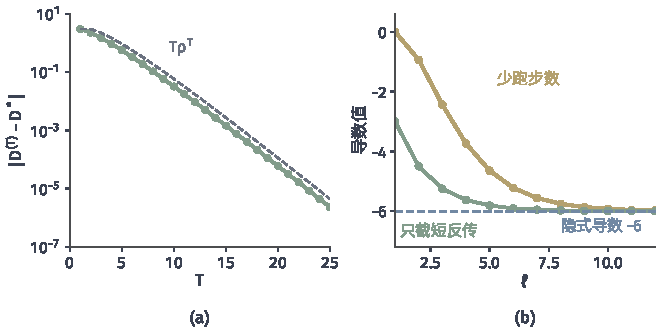
\includegraphics[width=112mm]{figures/05-optimization/07-multiple-criteria-and-nested-optimization/matplotlib/bilevel-unroll-derivative/figure.pdf}
 \caption{展开导数与隐式导数的关系，正则拟合例，$x=0$，$\alpha=1/2$。(a)绿线是导数误差$|D^{(T)}-D^\star|=3(T+1)2^{-T}$，虚线是定理~\ref{thm:bilevel-unroll-limit}型的参考界。(b)黄线是真实步数为$T=\ell$的完整展开导数，绿线是$T=20$、只反传$\ell$步的结果，蓝色虚线是隐式导数$-6$。}
 \label{fig:bilevel-unroll-derivative}
\end{BookInlineFigure}

截断后的向量一般不是$\Phi_T$的梯度，也不保证是它的下降方向。设误差向量为$\bm{e}$，真实梯度为$\bm{\gamma}$。只有在$\lVert\bm{e}\rVert_2<\lVert\bm{\gamma}\rVert_2$时才能由
\[
 \langle\bm{\gamma}+\bm{e},\bm{\gamma}\rangle\geq\lVert\bm{\gamma}\rVert_2\bigl(\lVert\bm{\gamma}\rVert_2-\lVert\bm{e}\rVert_2\bigr)>0
\]
断定它仍是下降方向。

\paragraph{与隐式微分的联系}
若内层已收敛，每一步的$\bm{A}^{(t)}$、$\bm{C}^{(t)}$都等于解点处的值$\bm{I}-\alpha\bm{H}$和$-\alpha\bm{B}$，反传$\ell$步给出
\[
 \nabla_{\bm{x}}F-\bm{B}^{\top}\Bigl[\alpha\sum_{k=0}^{\ell-1}(\bm{I}-\alpha\bm{H})^k\Bigr]\nabla_{\bm{y}}F.
\]
方括号正是式~\eqref{eq:bilevel-neumann}的前$\ell$项，所以截断反传相当于用Neumann级数的部分和代替$\bm{H}^{-1}$。

\subsection{极限关系}
\label{sec:bilevel-limit}

既然两种路线在内层收敛时形式一致，自然要问：$T\to\infty$时，展开的导数是否趋于隐式导数。答案是在收缩性等条件下成立，而只有迭代点收敛是不够的。

\begin{theorem}[展开导数的收敛]
\label{thm:bilevel-unroll-limit}
固定$\bm{x}$，内层用梯度下降，步长$\alpha\leq1/L_g$。设沿迭代路径和$\bm{y}^\star$处有$\mu\bm{I}\preceq\bm{H}\preceq L_g\bm{I}$，且存在常数$L_H,L_B$，使这些点上$\bm{H}$、$\bm{B}$关于$\bm{y}$分别$L_H$、$L_B$—Lipschitz。记
\begin{equation}
 \begin{gathered}
 \rho=1-\alpha\mu,\qquad\bm{D}^\star=-\bm{H}_\star^{-1}\bm{B}_\star,\\
 e_0=\lVert\bm{y}^{(0)}-\bm{y}^\star\rVert_2,\qquad c=\alpha(L_H\lVert\bm{D}^\star\rVert_2+L_B)e_0.
 \end{gathered}
 \label{eq:bilevel-unroll-constants}
\end{equation}
若迭代满足
\begin{equation}
 \lVert\bm{y}^{(t)}-\bm{y}^\star\rVert_2\leq\rho^te_0,
 \label{eq:bilevel-unroll-linear}
\end{equation}
则
\begin{equation}
 \lVert\bm{D}^{(T)}-\bm{D}^\star\rVert_2\leq\rho^T\lVert\bm{D}^{(0)}-\bm{D}^\star\rVert_2+cT\rho^{T-1}.
 \label{eq:bilevel-unroll-limit}
\end{equation}
\end{theorem}

\begin{proof}
先说明$\bm{D}^\star$是极限递推的不动点。把$\bm{A}_\star=\bm{I}-\alpha\bm{H}_\star$、$\bm{C}_\star=-\alpha\bm{B}_\star$代入，得到
\[
 \bm{A}_\star\bm{D}^\star+\bm{C}_\star=\bm{D}^\star-\alpha\bm{H}_\star\bm{D}^\star-\alpha\bm{B}_\star=\bm{D}^\star.
\]

记$\bm{E}^{(t)}=\bm{D}^{(t)}-\bm{D}^\star$，用递推式减去不动点方程，并在中间加减$\bm{A}^{(t)}\bm{D}^\star$，得到
\[
 \bm{E}^{(t+1)}=\bm{A}^{(t)}\bm{E}^{(t)}+(\bm{A}^{(t)}-\bm{A}_\star)\bm{D}^\star+(\bm{C}^{(t)}-\bm{C}_\star).
\]

条件$\alpha\leq1/L_g$使$\bm{A}^{(t)}$的特征值落在$[0,\rho]$，所以$\lVert\bm{A}^{(t)}\rVert_2\leq\rho$。由Lipschitz条件和式~\eqref{eq:bilevel-unroll-linear}，后两项的范数之和不超过$c\rho^t$，于是
\[
 \lVert\bm{E}^{(t+1)}\rVert_2\leq\rho\lVert\bm{E}^{(t)}\rVert_2+c\rho^t.
\]

对$T$归纳。$T=0$时式~\eqref{eq:bilevel-unroll-limit}成立。若对$T$成立，代入上式，得到
\[
 \lVert\bm{E}^{(T+1)}\rVert_2\leq\rho^{T+1}\lVert\bm{E}^{(0)}\rVert_2+cT\rho^{T}+c\rho^T=\rho^{T+1}\lVert\bm{E}^{(0)}\rVert_2+c(T+1)\rho^{T}.
\]
这就是$T+1$时的结论。
\end{proof}

收缩率$\rho$控制衰减，多出的因子$T$来自迭代点误差在每一层的累积。把结果代入式~\eqref{eq:bilevel-finite-gradient}，当$\nabla_{\bm{x}}F$、$\nabla_{\bm{y}}F$关于$\bm{y}$连续时，$\nabla\Phi_T\to\nabla\Phi$。

\paragraph{手算核对}
正则拟合例在$x=0$处，$\mu=L_g=1$，$\rho=1/2$，$L_H=0$，$L_B=1$，$e_0=3$，$c=3/2$，$\lVert D^{(0)}-D^\star\rVert=3$。式~\eqref{eq:bilevel-unroll-limit}的右端是$3\cdot2^{-T}+3T\cdot2^{-T}$。

另一方面，对式~\eqref{eq:bilevel-ridge-finite}直接求导，得到$D^{(T)}=-3+3(T+1)2^{-T}$，误差恰好等于
\[
 \lvert D^{(T)}-D^\star\rvert=3(T+1)2^{-T}.
\]
上界在这个例子里取等号。

\paragraph{点列收敛不够}
内层点列收敛这个事实本身，不足以交换求导与极限。设内层目标是$g=\frac12(y-x)^2$，$y^\star(x)=x$，某个带扰动的内层算法输出
\[
 y^{(T)}(x)=x+\frac{\sin(Tx)}{T}.
\]

对所有$x$，误差不超过$1/T$，点列一致收敛到内解。可是$\mathrm{d}y^{(T)}/\mathrm{d}x=1+\cos(Tx)$，在$x=0$处恒等于$2$，而隐式导数是$1$。误差的幅度在缩小，它的振荡频率却在增加，导数记录的恰恰是后者。定理~\ref{thm:bilevel-unroll-limit}用收缩和导数的Lipschitz条件排除了这种情形。

收缩一旦失去，结论也无从谈起。正则拟合例中$\alpha=1/2$时$q=(1-x)/2$，$x\geq3$时$\lvert q\rvert\geq1$，迭代不收敛，$\Phi_T$描述的是一个发散算法的输出。而且，固定的短展开并不自动给出真实双层目标的梯度：$T=2$时的导数$-15/16$与$-6$相差甚远。

\section{单层重述}
\label{sec:bilevel-single-level}

前两节都把$\Phi$当作函数，靠内层求解和求导来下降。另一种思路是不把内层嵌套着解，而把“$\bm{y}$确实是内解”写成关于$(\bm{x},\bm{y})$的约束，然后一起最小化外层目标。接下来要弄清：这样的约束有哪些写法，每种写法保留了什么，又失去了什么？

对乐观模型，由式~\eqref{eq:bilevel-optimistic-joint}，这个想法可以直接实现。悲观模型不行：外层目标里夹着一个对解集的$\sup$，把它改成对$\bm{y}$的联合最小化就等于把最坏情况换成了最好情况，它还需要再嵌套一层，不能套用下面的改写。本节只讨论乐观模型。

\subsection{最优性条件重述}
\label{sec:bilevel-kkt-reformulation}

用$\bm{y}$的最优性条件替代“$\bm{y}\in\bm{S}(\bm{x})$”是最直接的做法，内层有约束时这就是KKT条件。

\paragraph{写成一个单层问题}
沿用式~\eqref{eq:bilevel-lagrangian}的记号，把乘子也作为变量，得到下面的问题：
\begin{equation}
 \begin{aligned}
 \min_{\bm{x},\bm{y},\bm{\lambda},\bm{\nu}}\quad&F(\bm{x},\bm{y})\\
 \text{s.t.}\quad&\bm{x}\in\bm{C},\quad\nabla_{\bm{y}}\mathcal{L}=\bm{0},\quad\bm{h}=\bm{0},\\
 &\bm{c}\leq\bm{0},\quad\bm{\lambda}\geq\bm{0},\quad\lambda_ic_i=0,\ i=1,\ldots,m.
 \end{aligned}
 \label{eq:bilevel-mpcc}
\end{equation}
含有$\lambda_ic_i=0$这样的约束的问题称为\term{互补约束规划}（mathematical program with complementarity constraints），简称MPCC。

这样的改写要成立，必须保证KKT条件恰好刻画内层的全局解。KKT条件一般只是局部解的必要条件，下面的定理给出能作此替换的情形。

\begin{theorem}[凸内层的KKT重述]
\label{thm:bilevel-kkt-equivalence}
设对每个$\bm{x}\in\bm{C}$，$g(\bm{x},\cdot)$和$c_i(\bm{x},\cdot)$凸且连续可微，$h_j(\bm{x},\cdot)$仿射，内层满足Slater条件。则对每个$\bm{x}\in\bm{C}$，
\begin{equation}
 \bm{y}\in\bm{S}(\bm{x})\iff\text{存在}(\bm{\lambda},\bm{\nu})\text{使}(\bm{x},\bm{y},\bm{\lambda},\bm{\nu})\text{满足式~\eqref{eq:bilevel-mpcc}的约束}.
 \label{eq:bilevel-kkt-equivalence}
\end{equation}
于是$(\bm{x},\bm{y})$是乐观模型的全局解，当且仅当存在乘子使$(\bm{x},\bm{y},\bm{\lambda},\bm{\nu})$是式~\eqref{eq:bilevel-mpcc}的全局解。
\end{theorem}

\begin{proof}
固定$\bm{x}$。凸问题的KKT点是全局解，这给出“$\Leftarrow$”；Slater条件下凸问题的全局解满足KKT条件，乘子存在，这给出“$\Rightarrow$”。这两个结论见第~\ref{chap:constrained-optimality}章和第~\ref{chap:duality}章。两个问题的目标都只含$(\bm{x},\bm{y})$，可行点的$(\bm{x},\bm{y})$分量又相同，所以全局解的$(\bm{x},\bm{y})$分量也相同。
\end{proof}

定理只对应全局解。局部解的对应要复杂得多：式~\eqref{eq:bilevel-mpcc}的局部解固定了一组乘子，而原问题要比较所有乘子对应的邻近点，乘子不唯一时两者可以不一致。相关反例的构造较长，读者可查阅双层规划的专门文献。

\paragraph{非凸内层的反例}
内层非凸时，KKT点可能根本不是全局解。取无约束内层和外层
\[
 g(y)=\frac14y^4-\frac12y^2,\qquad F(y)=\frac12y^2.
\]

驻点方程$y^3-y=0$的解是$y\in\{-1,0,1\}$。全局解是$y=\pm1$，外层值是$1/2$。可是重述问题只要求驻点方程，它会选$y=0$，外层值是$0$，而$y=0$恰好是内层的局部极大点。

\paragraph{一个凸内层的例子}
取内层$\min_y\frac12(y-x)^2$，约束$y\geq0$，也就是$c=-y\leq0$。外层目标取$F=\frac12(x+1)^2+\frac12(y-1)^2$。内层的KKT条件是
\[
 y-x-\lambda=0,\qquad y\geq0,\qquad\lambda\geq0,\qquad\lambda y=0.
\]

互补条件把可行集分成两支。$\lambda=0$时$y=x\geq0$；$y=0$时$\lambda=-x\geq0$。这就是图~\ref{fig:bilevel-mpcc}(b)的折线，$y^\star(x)=\max\{x,0\}$。

在两支上分别求解。沿$y=x$，$x\geq0$，外层值是$x^2+1$，最小值是$x=0$处的$1$。沿$y=0$，$x\leq0$，外层值是$\frac12(x+1)^2+\frac12$，最小值是$x=-1$处的$\frac12$。全局解是$(x,y)=(-1,0)$。

\paragraph{互补约束为什么难}
图~\ref{fig:bilevel-mpcc}(a)画出了$a\geq0$、$b\geq0$、$ab=0$的可行集，它由两条半轴组成，没有内部，在原点还拐了一个直角。一般非线性规划算法依靠约束资格，而这类可行集恰好破坏它们。

\begin{BookInlineFigure}
 \centering
 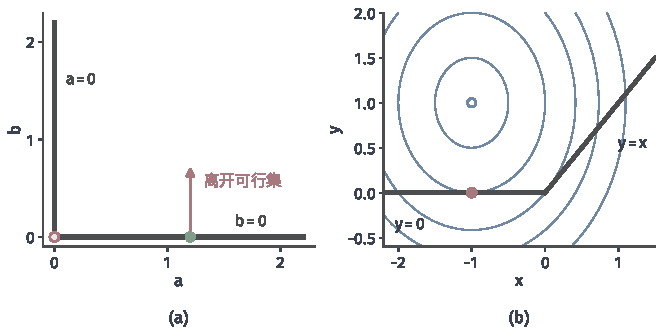
\includegraphics[width=112mm]{figures/05-optimization/07-multiple-criteria-and-nested-optimization/matplotlib/bilevel-mpcc/figure.pdf}
 \caption{互补约束的几何。(a)$a\geq0$、$b\geq0$、$ab=0$的可行集是两条半轴。在绿点处，严格满足不等式$b\geq0$的方向（红箭头）立刻离开可行集；原点处（空心点）拐角使等式约束的梯度为零。(b)内层$\min\frac12(y-x)^2$，$y\geq0$的解图像（深灰折线），蓝色是外层等高线，空心点是外层的无约束最小点$(-1,1)$，红点是双层问题的解$(-1,0)$。}
 \label{fig:bilevel-mpcc}
\end{BookInlineFigure}

\begin{lemma}[互补约束破坏MFCQ]
\label{lem:bilevel-mfcq-fails}
设$m\geq1$。式~\eqref{eq:bilevel-mpcc}的每个可行点都不满足Mangasarian—Fromovitz约束资格（MFCQ）。
\end{lemma}

\begin{proof}
MFCQ要求等式约束的梯度线性无关，并存在方向$\bm{d}$，使它与所有等式约束的梯度正交，且与所有活动不等式约束的梯度内积为负。考虑某一对约束$\lambda_i\geq0$、$c_i\leq0$、$e=\lambda_ic_i=0$，在全部变量构成的空间中，等式的梯度是
\[
 \nabla e=c_i\nabla\lambda_i+\lambda_i\nabla c_i.
\]

若$\lambda_i>0$，$c_i=0$，则$\nabla e=\lambda_i\nabla c_i$。$c_i\leq0$活动，MFCQ要求$\langle\nabla c_i,\bm{d}\rangle<0$，于是$\langle\nabla e,\bm{d}\rangle<0$，与正交矛盾。

若$\lambda_i=0$，$c_i<0$，则$\nabla e=c_i\nabla\lambda_i$。$-\lambda_i\leq0$活动，MFCQ要求$\langle\nabla\lambda_i,\bm{d}\rangle>0$，于是$\langle\nabla e,\bm{d}\rangle<0$，同样矛盾。

若$\lambda_i=c_i=0$，则$\nabla e=\bm{0}$，等式约束的梯度线性相关。三种情形穷尽了可行点的所有可能。
\end{proof}

所以即使内层是凸的，也不能把一般非线性规划的收敛结论直接搬过来，那些结论通常要求某种约束资格。实践中的做法有两类：内层约束不多时枚举互补的分支，每一支是一个正常的问题，但分支数最多是$2^m$；或者把$\lambda_ic_i=0$松弛成$-\lambda_ic_i\leq t$，让$t$逐渐趋于零，松弛问题有内部，但收敛到的点要回到原问题核对。

\subsection{值函数重述}
\label{sec:bilevel-value-reformulation}

最优性条件的重述要靠凸性才能表达全局最优。另一种写法直接比较目标值，不需要内层的结构。

\paragraph{直接比较内层目标值}
定义内层最优值函数
\begin{equation}
 V(\bm{x})=\inf_{\bm{y}\in\bm{Y}(\bm{x})}g(\bm{x},\bm{y}).
 \label{eq:bilevel-value-function}
\end{equation}
$\bm{y}$是内解，当且仅当它内层可行，且它的内层目标值达到了最优值。

\begin{lemma}[值函数重述]
\label{lem:bilevel-value-reformulation}
设$V(\bm{x})$有限。则
\begin{equation}
 \bm{y}\in\bm{S}(\bm{x})\iff\bm{y}\in\bm{Y}(\bm{x})\text{且}g(\bm{x},\bm{y})\leq V(\bm{x}).
 \label{eq:bilevel-value-constraint}
\end{equation}
\end{lemma}

\begin{proof}
若$\bm{y}\in\bm{S}(\bm{x})$，则$\bm{y}$可行且$g(\bm{x},\bm{y})=V(\bm{x})$。反过来，$\bm{y}$可行时必有$g(\bm{x},\bm{y})\geq V(\bm{x})$，再加上不等式$g(\bm{x},\bm{y})\leq V(\bm{x})$，就得到等号，所以$\bm{y}$取得内层最小值。
\end{proof}

引理没有用到任何凸性，所以全局选解这个要求被完整地写了下来。乐观模型因而等价于
\[
 \min_{\bm{x}\in\bm{C},\,\bm{y}\in\bm{Y}(\bm{x})}F(\bm{x},\bm{y})\quad\text{s.t.}\quad g(\bm{x},\bm{y})-V(\bm{x})\leq0.
\]

\paragraph{用正则拟合例计算}
把式~\eqref{eq:bilevel-ridge-solution}代入$g$并化简，得到
\[
 V(x)=\frac{9x}{2(1+x)}.
\]

$g$对$y$是二次函数，二次项系数为$(1+x)/2$，所以
\[
 g(x,y)-V(x)=\frac{1+x}{2}\bigl(y-y^\star(x)\bigr)^2.
\]
约束$g-V\leq0$迫使$y=y^\star(x)$，确实把内解曲线重新写了出来。$V$的导数可以用包络关系求，
\[
 V'(x)=\partial_xg(x,y^\star(x))=\frac12(y^\star)^2=\frac{9}{2(1+x)^2},
\]
它和直接求导的结果相同。

\paragraph{两个困难}
第一，$V$可能不光滑。式~\eqref{eq:bilevel-two-wells}的内层有$V(x)=-\lvert x\rvert$，在切换点$x=0$处有折点，如图~\ref{fig:bilevel-value}(a)。一般地，$V$是一族函数的下确界，切换解的地方就会出现折点。计算$V$本身也要解一次内层问题。

第二，约束本身是退化的。在$\bm{y}\in\bm{Y}(\bm{x})$上总有$g-V\geq0$，所以不存在严格满足$g-V<0$的点，Slater条件永远不成立。上面的例子里更明显：约束函数$\frac{1+x}{2}(y-y^\star)^2$在可行点处的梯度是零向量，它提供不了任何关于如何回到可行集的一阶信息。

\paragraph{松弛之后要重新核对}
常见的处理是把约束放宽成$g-V\leq\varepsilon$，$\varepsilon>0$。这样可行集有了内部，但代价是允许了不是内解的点。

正则拟合例中，$\varepsilon=0.1$时可行集成了内解曲线周围的一条带，它的半宽是$\sqrt{2\varepsilon/(1+x)}$，见图~\ref{fig:bilevel-value}(b)。外层目标在$y=1$处取最小值$0$，带子与直线$y=1$相交的部分全部是松弛问题的解。令$u=1+x$，条件是
\[
 (u-3)^2\leq0.2\,u.
\]

解得$u\in[2.319,3.881]$，即$x\in[1.319,2.881]$。真实的解$x=2$只是其中一点，松弛让最优解从一个点变成了一个区间，最优值也可能偏低。

\begin{BookInlineFigure}
 \centering
 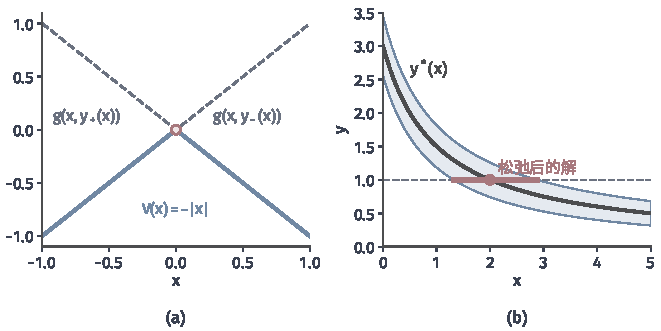
\includegraphics[width=112mm]{figures/05-optimization/07-multiple-criteria-and-nested-optimization/matplotlib/bilevel-value/figure.pdf}
 \caption{值函数重述的两个困难。(a)式~\eqref{eq:bilevel-two-wells}的最优值函数$V(x)=-|x|$（蓝），虚线是沿两条分支的内层值，切换点（空心点）处$V$不可微。(b)正则拟合例的松弛$g-V\leq0.1$：浅蓝带是松弛后的可行集，深灰线是内解，红色线段是带子与$y=1$的交集，即松弛问题的全部最优解；红点是原问题的解$x=2$。}
 \label{fig:bilevel-value}
\end{BookInlineFigure}

罚函数也可以用，把$\rho(g-V)$加进外层目标。有限的$\rho$得到的通常只是近似解。不论松弛还是惩罚，得到的点都要重新检查：内层最优间隙$g-V$有多大，它对应的内解距离有多大，以及改变$\varepsilon$或$\rho$后解是否稳定。

表~\ref{tab:bilevel-reformulations}比较两种重述。

\begin{BookInlineTable}
 \centering
 \begin{tabular}{lll}
  \toprule
  & KKT重述 & 值函数重述\\
  \midrule
  全局等价 & 需凸性与约束资格 & 不需要\\
  新增变量 & 乘子 & 无\\
  主要困难 & 互补约束 & $V$的计算与不光滑\\
  约束资格 & MFCQ处处失效 & Slater永不成立\\
  \bottomrule
 \end{tabular}
 \caption{乐观模型的两种单层重述。悲观模型不能这样改写。}
 \label{tab:bilevel-reformulations}
\end{BookInlineTable}

\section{外层求解}
\label{sec:bilevel-outer}

有了超梯度，外层就可以用前面各章的方法：$\bm{C}$是简单集合时用投影梯度（第~\ref{chap:feasible-iterations}章），变量多而问题光滑时用拟牛顿法（第~\ref{chap:quasi-newton}章），$\Phi$有折点时用非光滑方法（第~\ref{chap:nonsmooth-composite-optimization}章）。选择之前先要确定优化的是哪个目标：真实选解的$\Phi$，还是有限步的$\Phi_T$。

超梯度带着偏差时，外层能保证什么？若把带固定偏差的超梯度当成精确梯度，收敛结论就不成立了。下面按内层、导数、外层的顺序逐级核算。

\subsection{内层误差}
\label{sec:bilevel-inner-error}

内层算法停下时，手里是一个近似解$\hat{\bm{y}}$。这个点离内解有多远，可以用三个量来描述，它们含义不同，需要的计算条件也不同。

\paragraph{三种度量}
固定$\bm{x}$，记所选内解为$\bm{y}^\star$，定义
\[
 \delta=g(\bm{x},\hat{\bm{y}})-g(\bm{x},\bm{y}^\star),\qquad r=\lVert\nabla_{\bm{y}}g(\bm{x},\hat{\bm{y}})\rVert_2,\qquad d=\lVert\hat{\bm{y}}-\bm{y}^\star\rVert_2.
\]

$\delta$是内层目标差距，要知道最优值才能算。$r$是驻点残差，随手可算。$d$是到所选解的距离，通常没法直接算，而超梯度的误差恰恰取决于它。三者只有在特定条件下才能互相控制。

\begin{lemma}[强凸下的互控]
\label{lem:bilevel-inner-measures}
设对固定的$\bm{x}$，$\mu\bm{I}\preceq\nabla^2_{\bm{y}\bm{y}}g\preceq L_g\bm{I}$处处成立。则
\begin{align}
 \mu d&\leq r\leq L_gd,
 \label{eq:bilevel-inner-r}\\
 \frac{\mu}{2}d^2&\leq\delta\leq\frac{L_g}{2}d^2,
 \label{eq:bilevel-inner-delta}\\
 \frac{r^2}{2L_g}&\leq\delta\leq\frac{r^2}{2\mu}.
 \label{eq:bilevel-inner-pl}
\end{align}
\end{lemma}

\begin{proof}
记$\phi=g(\bm{x},\cdot)$，$\bm{e}=\hat{\bm{y}}-\bm{y}^\star$。由$\nabla\phi(\bm{y}^\star)=\bm{0}$和积分形式的中值定理，
\[
 \nabla\phi(\hat{\bm{y}})=\bar{\bm{H}}\bm{e},
\]
其中$\bar{\bm{H}}$是Hessian沿线段的平均，特征值在$[\mu,L_g]$内，这给出式~\eqref{eq:bilevel-inner-r}。

由Taylor公式，
\[
 \delta=\frac12\bm{e}^{\top}\tilde{\bm{H}}\bm{e},
\]
$\tilde{\bm{H}}$的特征值同样在$[\mu,L_g]$内，这给出式~\eqref{eq:bilevel-inner-delta}。

由强凸性，
\[
 \phi(\bm{y}^\star)\geq\phi(\hat{\bm{y}})-rd+\frac{\mu}{2}d^2\geq\phi(\hat{\bm{y}})-\frac{r^2}{2\mu},
\]
第二步是对$d$取最小，这给出式~\eqref{eq:bilevel-inner-pl}的右半。对左半，从$\hat{\bm{y}}$走一步梯度下降$\hat{\bm{y}}-\nabla\phi(\hat{\bm{y}})/L_g$，由下降引理，函数值至少下降$r^2/(2L_g)$，而它不会低于$\phi(\bm{y}^\star)$。
\end{proof}

\paragraph{条件去掉会怎样}
图~\ref{fig:bilevel-inner-measures}对比了强凸的$g=y^2/2$和平坦的$g=y^4/4$。对后者，$r=d^3$，$\delta=d^4/4$。当$d=0.1$时，残差只有$10^{-3}$，目标差距只有$2.5\times10^{-5}$，看上去已经收敛得很好，到解的距离却还有$0.1$。

\begin{BookInlineFigure}
 \centering
 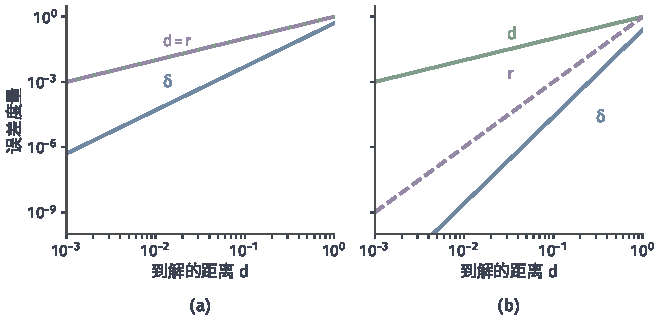
\includegraphics[width=112mm]{figures/05-optimization/07-multiple-criteria-and-nested-optimization/matplotlib/bilevel-inner-measures/figure.pdf}
 \caption{三种内层误差度量随距离$d$的变化，双对数坐标。(a)强凸的$g=y^2/2$：残差$r$（紫色虚线）与$d$（绿）重合，目标差距$\delta$（蓝）是$d^2/2$。(b)平坦的$g=y^4/4$：$r=d^3$，$\delta=d^4/4$，残差和目标差距都远小于到解的距离。}
 \label{fig:bilevel-inner-measures}
\end{BookInlineFigure}

非凸时情况更糟。$r=0$只说明是驻点，它可能是极大点或鞍点。即使是极小点，$d$也必须对着“所选解”算：$\delta$和$r$再小，也无法说明算法是否在正确的那个碗里。

\paragraph{热启动的得失}
外层变化不大时，内层从上一轮解继续，可以省去大量迭代，这是热启动的好处。第~\ref{sec:bilevel-switching}小节也展示了它的代价：它会一直追踪同一条局部分支，穿过切换点也不察觉。热启动减少重复求解，但不能免除全局选解的核对；内层非凸时，需要定期从不同初值重解内层，比较内层目标值。

\subsection{导数误差}
\label{sec:bilevel-derivative-error}

超梯度的误差有几个来源：内解没解准，所有二阶导数都算在错误的点上；伴随方程没解准；或者反传被截断。它们对外层方向的影响要分开看。

\paragraph{两项误差的分解}
记$\hat{\bm{H}}$、$\hat{\bm{B}}$是在$\hat{\bm{y}}$处计算的矩阵，$\bm{f}(\bm{y})=\nabla_{\bm{y}}F(\bm{x},\bm{y})$，并简写$\hat{\bm{f}}=\bm{f}(\hat{\bm{y}})$、$\bm{f}_\star=\bm{f}(\bm{y}^\star)$。设$\tilde{\bm{v}}$是伴随方程的近似解，残差和超梯度估计分别是
\begin{equation}
 \bm{r}_{\bm{v}}=\hat{\bm{H}}\tilde{\bm{v}}-\hat{\bm{f}},\qquad\hat{\bm{\gamma}}=\nabla_{\bm{x}}F(\bm{x},\hat{\bm{y}})-\hat{\bm{B}}^{\top}\tilde{\bm{v}}.
 \label{eq:bilevel-hypergradient-estimate}
\end{equation}

\begin{theorem}[超梯度误差的分解]
\label{thm:bilevel-hypergradient-error}
固定$\bm{x}$，设在$\bm{y}^\star$和$\hat{\bm{y}}$之间：$\bm{H}\succeq\mu\bm{I}$，$\lVert\hat{\bm{B}}\rVert_2\leq M_B$，$\lVert\bm{f}_\star\rVert_2\leq M_F$；$\nabla_{\bm{x}}F$、$\nabla_{\bm{y}}F$关于$\bm{y}$是$L_F$—Lipschitz的，$\bm{H}$、$\bm{B}$关于$\bm{y}$分别是$L_H$、$L_B$—Lipschitz的。记$d=\lVert\hat{\bm{y}}-\bm{y}^\star\rVert_2$。则
\begin{equation}
 \lVert\hat{\bm{\gamma}}-\nabla\Phi(\bm{x})\rVert_2\leq C_d\,d+\frac{M_B}{\mu}\lVert\bm{r}_{\bm{v}}\rVert_2,
 \label{eq:bilevel-hypergradient-error}
\end{equation}
其中常数为
\begin{equation}
 C_d=L_F+\frac{L_BM_F}{\mu}+\frac{M_B}{\mu}\Bigl(L_F+\frac{L_HM_F}{\mu}\Bigr).
 \label{eq:bilevel-hypergradient-constant}
\end{equation}
\end{theorem}

\begin{proof}
记$\bm{v}^\star=\bm{H}_\star^{-1}\bm{f}_\star$，由$\bm{H}_\star\succeq\mu\bm{I}$得$\lVert\bm{v}^\star\rVert_2\leq M_F/\mu$。在$\bm{B}$的差上加减一项，把误差拆成三部分：
\[
 \begin{aligned}
 \hat{\bm{\gamma}}-\nabla\Phi={}&\bigl[\nabla_{\bm{x}}F(\bm{x},\hat{\bm{y}})-\nabla_{\bm{x}}F(\bm{x},\bm{y}^\star)\bigr]\\
 &-(\hat{\bm{B}}-\bm{B}_\star)^{\top}\bm{v}^\star-\hat{\bm{B}}^{\top}(\tilde{\bm{v}}-\bm{v}^\star).
 \end{aligned}
\]

前两部分的范数分别不超过$L_Fd$和$L_BM_Fd/\mu$。第三部分要估计$\tilde{\bm{v}}-\bm{v}^\star$。由残差的定义和$\bm{f}_\star=\bm{H}_\star\bm{v}^\star$，得到
\[
 \hat{\bm{H}}(\tilde{\bm{v}}-\bm{v}^\star)=\bm{r}_{\bm{v}}+(\hat{\bm{f}}-\bm{f}_\star)-(\hat{\bm{H}}-\bm{H}_\star)\bm{v}^\star.
\]

两边乘$\hat{\bm{H}}^{-1}$并取范数，得到
\[
 \lVert\tilde{\bm{v}}-\bm{v}^\star\rVert_2\leq\frac{1}{\mu}\Bigl(\lVert\bm{r}_{\bm{v}}\rVert_2+L_Fd+\frac{L_HM_F}{\mu}d\Bigr).
\]
再乘$\lVert\hat{\bm{B}}\rVert_2\leq M_B$，三部分相加即得式~\eqref{eq:bilevel-hypergradient-error}。
\end{proof}

右端第一项由内层距离$d$负责，第二项由伴随残差负责，两者互不替代。只把$d$压小而不解准伴随方程，或者反过来，都会停在另一项决定的误差水平上。迭代展开时第二项换成式~\eqref{eq:bilevel-truncation}的截断误差。这些结论都要有相应的稳定性条件：$\mu$变小，所有系数都变大；$\bm{H}$奇异时上界不成立。

\paragraph{手算一次}
正则拟合例在$x=1$处，$y^\star=3/2$，$\Phi'(1)=-3/8$。设内层只解到$\hat{y}=1.4$，$d=0.1$，这时$\hat{H}=2$，$\hat{B}=1.4$，$\partial_yF=0.4$。伴随方程精确解是$\hat{v}=0.2$，超梯度估计和误差分别是
\[
 \hat{\gamma}=-0.28,\qquad\lvert\hat{\gamma}-\Phi'(1)\rvert=0.095.
\]

若再把伴随方程解错，取$\tilde{v}=0.15$，残差是$r_v=2\times0.15-0.4=-0.1$，则
\[
 \tilde{\gamma}=-0.21,\qquad\lvert\tilde{\gamma}-\Phi'(1)\rvert=0.165.
\]

代入式~\eqref{eq:bilevel-hypergradient-constant}。这里$L_F=L_B=1$，$L_H=0$，$\mu=2$，$M_F=1/2$，$M_B=1.4$，所以$C_d=1.95$，式~\eqref{eq:bilevel-hypergradient-error}的右端是
\[
 1.95\times0.1+0.7\times0.1=0.265.
\]
它确实是$0.165$的上界。

\paragraph{用数值实验看两项}
图~\ref{fig:bilevel-error-grid}用一个$d=30$的正则最小二乘内层，同时改变内层步数$K$和共轭梯度步数$k$。(a)中$k$固定时，增加$K$只能把误差压到某个平台，平台高度由$k$决定。(b)中$K$固定时，增加$k$也只能压到由$K$决定的平台。两个旋钮要一起拧，单独加大其中一个是浪费。

\begin{BookInlineFigure}
 \centering
 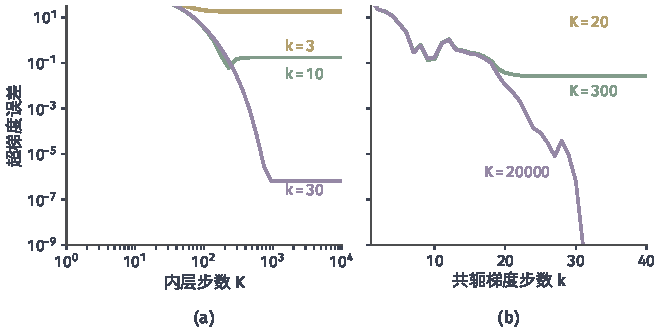
\includegraphics[width=112mm]{figures/05-optimization/07-multiple-criteria-and-nested-optimization/matplotlib/bilevel-error-grid/figure.pdf}
 \caption{超梯度误差的两个来源。内层是$d=30$的正则最小二乘，$x=0.05$，$\kappa\approx48$，数据由固定种子生成；内层用从零出发的梯度下降，步长$1/L_g$，伴随方程用共轭梯度法。(a)固定$k=3,10,30$，误差随内层步数$K$的变化。(b)固定$K=20,300,20000$，误差随共轭梯度步数$k$的变化。}
 \label{fig:bilevel-error-grid}
\end{BookInlineFigure}

\subsection{外层误差}
\label{sec:bilevel-outer-error}

最后把内层和导数的误差接到外层。本小节要解决的问题是：外层迭代用的是有偏差的超梯度，最终能保证什么，以及什么时候应该停下。

\paragraph{主要思想：偏差决定下限}
外层最简单的情形是无约束的梯度下降，用带误差$\bm{e}^{(t)}$的估计代替真实梯度：
\[
 \hat{\bm{\gamma}}^{(t)}=\nabla\Phi(\bm{x}^{(t)})+\bm{e}^{(t)}.
\]
下面的定理说明，偏差会直接进入驻定精度。

\begin{theorem}[带误差的外层梯度下降]
\label{thm:bilevel-inexact-outer}
设$\Phi$有下界$\Phi_{\inf}$，梯度在含迭代点的区域上$L_{\Phi}$—Lipschitz。迭代
\begin{equation}
 \bm{x}^{(t+1)}=\bm{x}^{(t)}-\frac{1}{L_{\Phi}}\hat{\bm{\gamma}}^{(t)}
 \label{eq:bilevel-outer-update}
\end{equation}
满足
\begin{equation}
 \min_{0\leq t<T}\lVert\nabla\Phi(\bm{x}^{(t)})\rVert_2^2\leq\frac{2L_{\Phi}\bigl(\Phi(\bm{x}^{(0)})-\Phi_{\inf}\bigr)}{T}+\frac1T\sum_{t=0}^{T-1}\lVert\bm{e}^{(t)}\rVert_2^2.
 \label{eq:bilevel-inexact-outer}
\end{equation}
\end{theorem}

\begin{proof}
记$\bm{\gamma}=\nabla\Phi(\bm{x}^{(t)})$，$\hat{\bm{\gamma}}=\bm{\gamma}+\bm{e}$，略去上标。由下降引理，
\[
 \Phi(\bm{x}^{(t+1)})\leq\Phi(\bm{x}^{(t)})-\frac{1}{L_{\Phi}}\langle\bm{\gamma},\hat{\bm{\gamma}}\rangle+\frac{1}{2L_{\Phi}}\lVert\hat{\bm{\gamma}}\rVert_2^2.
\]

利用恒等式
\[
 2\langle\bm{\gamma},\hat{\bm{\gamma}}\rangle=\lVert\bm{\gamma}\rVert_2^2+\lVert\hat{\bm{\gamma}}\rVert_2^2-\lVert\bm{e}\rVert_2^2,
\]
$\lVert\hat{\bm{\gamma}}\rVert_2^2$项正好抵消，得到
\[
 \Phi(\bm{x}^{(t+1)})\leq\Phi(\bm{x}^{(t)})-\frac{1}{2L_{\Phi}}\lVert\bm{\gamma}\rVert_2^2+\frac{1}{2L_{\Phi}}\lVert\bm{e}\rVert_2^2.
\]

对$t$从$0$到$T-1$求和，用$\Phi(\bm{x}^{(T)})\geq\Phi_{\inf}$，两边乘$2L_{\Phi}/T$，再用最小值不超过平均值即得。
\end{proof}

若偏差始终约为$\varepsilon$，式~\eqref{eq:bilevel-inexact-outer}右端第二项约为$\varepsilon^2$，不随$T$减小，这个上界只能保证$\lVert\nabla\Phi\rVert_2$降到$\varepsilon$的量级。要得到收敛，内层精度必须随外层进展提高，比如让$\sum_t\lVert\bm{e}^{(t)}\rVert_2^2$有限，这时第二项按$1/T$衰减。

这正对应图~\ref{fig:bilevel-outer-bias}。正则拟合例取$\eta=1$，从$x^{(0)}=1$出发，内层跑固定的$K$步后代入隐式公式。$K=2$时迭代收敛到$x=5/3$，这里$\hat{y}=1$，估计的超梯度为零，真实梯度却是$-27/512$。$K$增大时偏差缩小但不消失，只有$K$随$t$增长时才收敛到$x=2$。

\begin{BookInlineFigure}
 \centering
 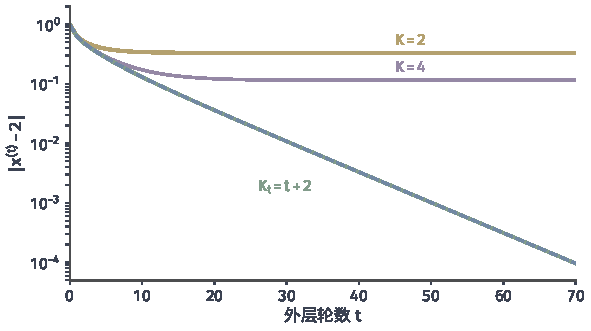
\includegraphics[width=100mm]{figures/05-optimization/07-multiple-criteria-and-nested-optimization/matplotlib/bilevel-outer-bias/figure.pdf}
 \caption{外层迭代误差$\lvert x^{(t)}-2\rvert$，正则拟合例，外层步长$\eta=1$，$x^{(0)}=1$，内层每轮从$y^{(0)}=0$跑$K$步后用隐式公式。黄线$K=2$、紫线$K=4$停在偏差决定的平台，绿线$K_t=t+2$与精确内解（蓝色虚线）几乎重合，持续收敛。}
 \label{fig:bilevel-outer-bias}
\end{BookInlineFigure}

\paragraph{计算过程}
把整个外层循环在这个例子上走几轮，内层步数取$K_t=t+2$。

\needspace{6\baselineskip}
\paragraph{变量}
\begin{itemize}
 \item 外层迭代点$x^{(t)}$，外层步长$\eta$。
 \item 内层输出$\hat{y}$，内层残差$r=(1+x)\hat{y}-3$。
 \item 伴随解$v$，超梯度估计$\hat{\gamma}$。
\end{itemize}

\paragraph{初始化}
例中$x^{(0)}=1$，$\eta=1$。正则拟合例在$x\geq1$上$\lvert\Phi''\rvert\leq15/16$，步长$\eta=1$略小于$1/L_{\Phi}=16/15$，定理~\ref{thm:bilevel-inexact-outer}的证明同样适用，只需把$L_{\Phi}$换成$1/\eta$。

\needspace{6\baselineskip}
\paragraph{每轮更新}
\begin{enumerate}
 \item 内层从$y^{(0)}=0$运行$K_t$步，由式~\eqref{eq:bilevel-ridge-finite}得到$\hat{y}$，并记录残差$r$。

 例中第一轮$x=1$，$q=0$，$\hat{y}=3/2$，残差为$0$。

 \item 解伴随方程，由式~\eqref{eq:bilevel-hypergradient-estimate}得到超梯度估计。

 例中$H=1+x$，$\partial_yF=\hat{y}-1$，$B=\hat{y}$，第一轮的结果是
 \[
  v=\frac{\hat{y}-1}{1+x}=\frac14,\qquad\hat{\gamma}=-\hat{y}v=-\frac38.
 \]

 \item 更新外层变量：$x^{(t+1)}=x^{(t)}-\eta\hat{\gamma}$。

 例中第一轮得到$x^{(1)}=11/8=1.375$。后面几轮的数值见表~\ref{tab:bilevel-outer-rounds}。
\end{enumerate}

\begin{BookInlineTable}
 \centering
 \begin{tabular}{rrrrrrr}
  \toprule
  $t$ & $K_t$ & $x^{(t)}$ & $\hat{y}$ & $r$ & $\hat{\gamma}$ & $\Phi'$\\
  \midrule
  $0$ & $2$ & $1.0000$ & $1.5000$ & $0.0000$ & $-0.3750$ & $-0.3750$\\
  $1$ & $3$ & $1.3750$ & $1.2715$ & $0.0198$ & $-0.1453$ & $-0.1400$\\
  $2$ & $4$ & $1.5203$ & $1.1849$ & $-0.0137$ & $-0.0869$ & $-0.0899$\\
  $3$ & $5$ & $1.6072$ & $1.1536$ & $0.0077$ & $-0.0680$ & $-0.0665$\\
  $4$ & $6$ & $1.6752$ & $1.1197$ & $-0.0044$ & $-0.0501$ & $-0.0509$\\
  \bottomrule
 \end{tabular}
 \caption{正则拟合例的外层循环，$\eta=1$，内层步数$K_t=t+2$。最后一列是在当前$x^{(t)}$处的真实超梯度。}
 \label{tab:bilevel-outer-rounds}
\end{BookInlineTable}

最终$x^{(t)}$趋于$x=2$。表中$\hat{\gamma}$与真实导数的差随内层残差缩小，这就是定理~\ref{thm:bilevel-hypergradient-error}所说的情况。

\paragraph{报告什么、何时停止}
外层的停止不能只看损失曲线，下面四项要分别检查，其中任何一项不达标都不能得出结论。

\begin{itemize}
 \item 外层可行性：$\bm{x}\in\bm{C}$是否成立，$\bm{x}$是否在$\operatorname{dom}\bm{S}$内，也就是内层确实有解。
 \item 外层驻定：有约束时用投影梯度的残差，无约束时用$\lVert\hat{\bm{\gamma}}\rVert_2$，并以估计的偏差为基准；$\lVert\hat{\bm{\gamma}}\rVert_2$低于偏差水平时继续迭代已没有依据。
 \item 内层误差：驻点残差或目标差距；非凸时再比较不同初值下的内层目标值。
 \item 导数误差：伴随残差或截断长度，并可用$\Phi$的中心差分抽查几个方向，差分时内层要解得足够准。
\end{itemize}

\paragraph{成本核算}
总成本要把四个部分分开算。设外层跑$T_{\mathrm{o}}$轮，每轮内层$K$步、共轭梯度$k$步，内层梯度的成本记作一个单位，Hessian向量积是它的常数倍。隐式微分的总计算量约是$T_{\mathrm{o}}(K+ck)$个单位，$c$是这个常数倍数，存储是$O(d)$。反向展开的计算量约是$cT_{\mathrm{o}}K$，存储变成$O(Kd)$，用检查点可以再压缩。内层病态时$K$和$k$都要增大，这是这类方法最主要的成本。

\paragraph{局部结论与全局结论}
定理~\ref{thm:bilevel-inexact-outer}只保证驻定，而$\Phi$一般是非凸的。即使内层对$y$强凸、外层对$y$凸，$\Phi$也可能非凸：正则拟合例有
\[
 \Phi''(x)=\frac{27-6u}{u^4},\qquad u=1+x,
\]
在$x>7/2$时为负。内层非凸时问题更严重，第~\ref{sec:bilevel-switching}小节的例子中$\Phi$还会跳变。所以局部收敛的结果，加上驻定残差很小，都不能自动说成整个双层问题的全局最优。要作全局的声明，需要多初值搜索或问题本身的结构，并如实说明已检查的范围。

\section{本章小结}
\label{sec:bilevel-summary}

双层优化的外层目标要读取一次优化的结果。本章首先分清三种对象：内解唯一时的$\Phi$，多解时靠规则确定的$\Phi_{\mathrm{o}}$和$\Phi_{\mathrm{p}}$，以及运行有限步算法得到的$\Phi_T$。乐观模型在紧性和连续性下有解，悲观模型没有同样的保证，算法的隐含择解不自动等于其中任何一种。内层无解的$\bm{x}$要排除，不能使用算法在那里给出的数字。

对解映射，Hessian正定给出局部的可微分支，全局强凸才让分支代表唯一的内解。驻点Jacobian可逆只保证有驻点分支，不保证是极小点；内解唯一也不保证可微。非凸内层的全局选解可能跳变，外层目标跟着不连续，算法沿分支算出的导数穿过切换点后就不再描述全局选解。

求导有两条路线。隐式微分在解点处解一个伴随方程，得到$\nabla\Phi=\nabla_{\bm{x}}F-\bm{B}^{\top}\bm{v}$，第二项是内解的响应，内层病态时线性残差被$1/\mu$放大；约束内层要解KKT系统，活动集变化、严格互补失效或KKT矩阵奇异时这个公式不能用。迭代展开对算法输出求导，得到的是$\Phi_T$的精确导数，反向累积省去大矩阵但要保存轨迹，截断反传则是导数的近似。

两条路线的关系由定理~\ref{thm:bilevel-unroll-limit}回答：内层一致收缩且二阶导数Lipschitz时，展开导数以$T\rho^T$的速率趋于隐式导数；只有点列收敛不够，固定的短展开也不是真实目标的梯度。

单层重述把内层最优性变成约束。KKT重述在凸内层和约束资格下全局等价，但产生的互补约束使MFCQ处处失效；值函数重述不需要凸性，代价是$V$可能不光滑、约束退化，松弛后要重新核对等价性。悲观模型不能这样改写。

表~\ref{tab:bilevel-summary}按误差来源归纳要核对的内容。外层收敛的曲线只回答了最后一行，其余各行需要各自的证据；局部驻定也不等于全局最优。

\begin{BookInlineTable}
 \centering
 \begin{tabular}{lll}
  \toprule
  误差来源 & 度量 & 控制手段\\
  \midrule
  内层求解 & $\delta$、$r$、$d$ & 增加内层步数\\
  内层选解 & 不同初值的内层值 & 重解，勿仅靠热启动\\
  伴随或截断 & $\lVert\bm{r}_{\bm{v}}\rVert_2$、$\ell$ & 增加线性迭代或反传长度\\
  外层 & 驻定残差、可行性 & 增加轮数，内层精度递增\\
  \bottomrule
 \end{tabular}
 \caption{双层求解中需要分别核对的四类误差。}
 \label{tab:bilevel-summary}
\end{BookInlineTable}

